\documentclass[journal,twoside,web]{ieeecolor}
\usepackage{tmi}
\usepackage{cite}
\usepackage{amsmath,amssymb,amsfonts}
\usepackage{algorithmic}
\usepackage{graphicx}
\usepackage{textcomp}

% my package
\usepackage{multirow} 
\usepackage{tabularx}
\usepackage{pifont}
\usepackage{booktabs}
\usepackage{makecell} % 可选，用于更灵活的换行

\usepackage{booktabs}
\usepackage{setspace}

\usepackage{dblfloatfix} % 大图放置

\def\BibTeX{{\rm B\kern-.05em{\sc i\kern-.025em b}\kern-.08em
    T\kern-.1667em\lower.7ex\hbox{E}\kern-.125emX}}
\markboth{\journalname, VOL. XX, NO. XX, XXXX 2020}
{Author \MakeLowercase{\textit{et al.}}: Preparation of Papers for IEEE TRANSACTIONS ON MEDICAL IMAGING}
\begin{document}
\title{Few-Shot Distillation for Real-time Surgical Phase Recognition under Label Scarcity}

\author{Minqing Zhang, Second B. Author,and Wu Yuan, \IEEEmembership{Senior Member, IEEE} 
\thanks{This paragraph of the first footnote will contain the date on which
you submitted your paper for review. It will also contain support information,
including sponsor and financial support acknowledgment. For example, 
``This work was supported in part by the U.S. Department of Commerce under Grant BS123456.'' }
\thanks{The next few paragraphs should contain the authors' current affiliations,
including current address and e-mail. For example, F. A. Author is with the
National Institute of Standards and Technology, Boulder, CO 80305 USA (e-mail:author@boulder.nist.gov). }
\thanks{S. B. Author, Jr., was with Rice University, Houston, TX 77005 USA.
He is now with the Department of Physics, Colorado State University,
Fort Collins, CO 80523 USA (e-mail: author@lamar.colostate.edu).}
\thanks{T. C. Author is with the Electrical Engineering Department,
University of Colorado, Boulder, CO 80309 USA, on leave from the National
Research Institute for Metals, Tsukuba, Japan (e-mail: author@nrim.go.jp).}}

\maketitle

\begin{abstract}
As surgical phase recognition (SPR) enters the foundation model (FM) era, the FM paradigm itself exposes two clinical deficiencies: it relies on massive training data that is prohibitive to curate in surgery, and its heavy architectures cannot sustain the real-time inference that clinical deployment demands. Our pilot study further shows that, under few-shot SPR, generic FMs match or outperform specialized surgical FMs, indicating that the data deficiency can be sidestepped rather than satisfied. We therefore build on a generic visual prior and present a redundancy-aware framework that turns the dual redundancy of surgical videos---dominant background regions and repetitive steady-state frames---from an obstacle into an inductive bias under scarce supervision. First, to break the FM paradigm's reliance on massive data, we introduce SPR-Teacher, a spatiotemporal adaptation tuning framework that adapts a frozen generic image FM to surgical video with only a handful of labeled videos: salient spatial token selection (SSTS) compresses spatial redundancy through a soft top-$K$ saliency gate, and keyframe-prior temporal fusion (KPTF) compresses temporal redundancy by aggregating the most discriminative moments. Second, to cure the real-time deficiency, we propose an architecture-agnostic distillation strategy that compresses SPR-Teacher into SPR-Lite, a lightweight student family for arbitrary backbones: a cross-attention projection bridges heterogeneous student feature maps into the teacher's token space, and a spatiotemporally-guided distillation transfers the teacher's where- and when-to-look priors as dense supervision to compensate for the scarce labels. Comprehensive experiments on five SPR datasets, including four public benchmarks and one private clinical cohort, demonstrate that SPR-Teacher substantially outperforms state-of-the-art methods in few-shot scenarios, and SPR-Lite approaches this performance with under 9 million parameters at over 25\,FPS on a single CPU.
\end{abstract}

\begin{IEEEkeywords}
Surgical phase recognition, few-shot learning, knowledge distillation, real-time deployment.
\end{IEEEkeywords}

\section{Introduction}
\label{sec:introduction}
%%%%%%%%%%%%% 我们干了啥事 %%%%%%%%%%%%
% 1.在 few-shot SPR 上对 generic/surgical FM 做了简单对比，发现 generic FM（DINOv3）潜力很大
% 2.选择DINOv3作为generic FM，然后针对性设计了video适配的策略
% 3.考虑临床部署挑战，提出了异构蒸馏策略
% 4.我们实验丰富，public和private数据集都验证few-shot优势明显，实时性部分也极大提升

% 总结三大卖点：generic FM 适配、few-shot即可高acc、计算效率实时性轻量化
%%%%%%%%%%%%%%%%%%%%%%%%%%%%%%%%%%%%%%%%%%%%%


\IEEEPARstart{S}{urgical} phase recognition (SPR), which identifies frame-wise surgical intentions from procedural videos, is foundational for intelligent operating rooms by supporting intraoperative decision support~\cite{vermeulen2023ultra}, real-time anomaly detection~\cite{mithany2023advancements}, and postoperative skill assessment~\cite{cao2023intelligent}. 
Recently, the domain has shifted toward pre-training surgical foundation models (FMs) on expansive corpora~\cite{batic2024endovit,yang2026large,wu2026surgmotion}, demonstrating promising performance. 
However, this relentless scaling introduces key clinical barriers that remain under-addressed. On one hand, curating massive surgical datasets incurs prohibitive annotation costs, privacy risks, and procedural biases. On the other hand, the associated parameter explosion renders heavy architectures computationally infeasible for resource-constrained clinical hardware. Crucially, practical SPR demands real-time inference, as instant intraoperative feedback directly impacts patient safety. Consequently, amid the push for larger surgical FMs, simultaneously overcoming heavy data reliance and deployment latency remains a critical yet overlooked challenge for practical SPR.

To address the data burden, general visual FMs offer a promising avenue by leveraging rich pretrained representations for downstream adaptation under limited supervision. Generic FMs have evolved rapidly across image and video domains, spanning self-supervised frameworks such as DINOv3~\cite{simeoni2025dinov3} and VideoMAEv2~\cite{wang2023videomae} alongside vision-language contrastive models like CLIP~\cite{radford2021learning} and InternVideo2~\cite{wang2024internvideo2}. Intriguingly, our systematic evaluation across five surgical datasets reveals that generic FMs match or outperform specialized surgical FMs in few-shot scenarios, despite lacking surgical pretraining exposure. Motivated by this observation, we select DINOv3 as the backbone and propose DINO-SPR, a novel spatiotemporal adaptation framework for few-shot settings. By incorporating salient spatial token selection (SSTS) and keyframe-prior temporal fusion (KPTF), DINO-SPR filters irrelevant background while preserving discriminative moments for effective video understanding. Consequently, with only a handful of labeled videos, this adaptation unlocks the strong potential of generic FMs for SPR without relying on massive surgical corpora.

Although DINO-SPR demonstrates remarkable data efficiency, its reliance on a heavy ViT backbone introduces heavy computational overhead and rigid deployment constraints. To overcome this bottleneck, we propose an architecture-agnostic distillation strategy that transfers the teacher into DINO-SPR Lite. To bridge the teacher-student structural discrepancy, a cross-attention projection (CAP) maps heterogeneous student feature maps into the teacher's token space, enabling flexible supervision across CNN, ViT, and hybrid architectures. Complementing this alignment, a spatiotemporally-guided distillation (STGD) transfers spatial and temporal priors into intermediate student representations, supplying the dense supervisory signals missing under scarce annotations. As shown in Fig.~\ref{fig:tradeoff}, the resulting DINO-SPR Lite models across three diverse student families achieve real-time CPU inference while approaching teacher-level accuracy, successfully reconciling accuracy and speed for clinical deployment.


\begin{figure}[t]
\centerline{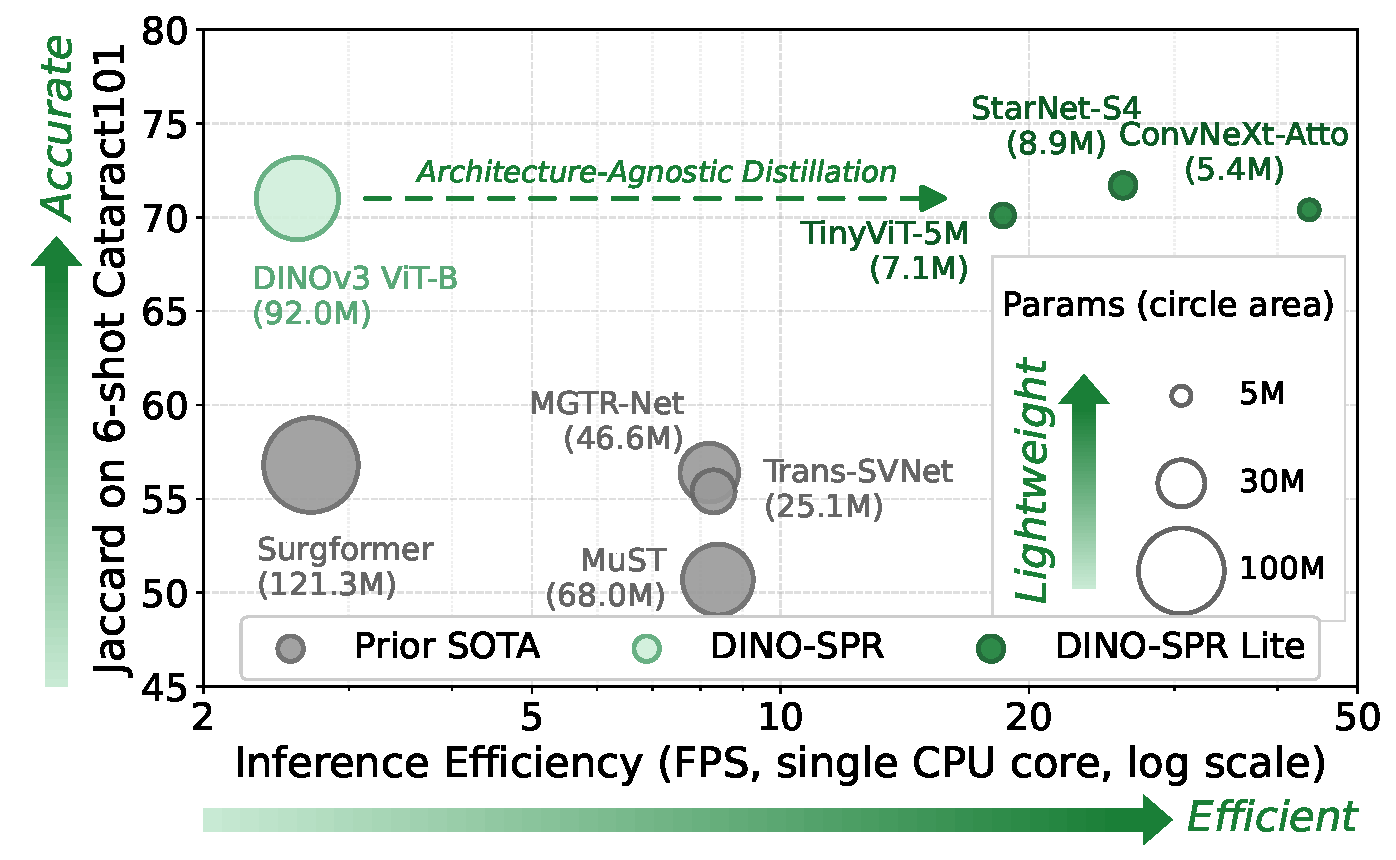
\includegraphics[width=\columnwidth]{resources/fig_computational_cost.pdf}}
\caption{6-shot Cataract101 Jaccard against inference efficiency on CPU, with circle area proportional to parameter count. Prior methods (gray) stay below 8.4\,FPS, while the DINO-SPR Lite students (dark green) match the DINO-SPR teacher (light green) at 18.6 to 43.7\,FPS.}
\label{fig:tradeoff}
\end{figure}


Our contributions could be summarized as follow:
% 贡献1：在 few-shot SPR 上对 representative 的 generic/surgical FM 做了简单对比，发现 generic FM DINOv3 的 few-shot 泛化潜力很大，由此选定 backbone
% 我们设计了video adaptation的策略，把image-based的DINOv3模型快速适配到surgical video任务
% 我们提出了异构模型蒸馏的方法，将few-shot适配后的DINOv3蒸馏到不同架构的轻量化模型，极大地提升了临床部署效率
% 5个手术阶段识别数据集，其中包含一个私有数据集，广泛验证了我们的算法，在few-shot场景下的准确率表现大幅超越previous SOTAs，并且在轻量化部署方面也明显更优
\begin{enumerate}
    \item We benchmark representative visual FMs on few-shot SPR and find that the
    generic DINOv3, although barely exposed to surgical data, already shows
    strong generalization, which motivates our choice of backbone.
    \item We devise a spatiotemporal adaptation tuning for DINOv3. The proposed SSTS and KPTF
    modules concentrate on the discriminative regions and key moments, enabling
    accurate adaptation under few-shot settings.
    \item We propose an architecture-agnostic distillation that compresses
    DINO-SPR into a lightweight student of any backbone, enabling flexible and real-time deployment.
    \item Extensive experiments show that DINO-SPR substantially surpasses previous
    state-of-the-art under few-shot settings, and DINO-SPR Lite retains this
    performance with fewer parameters and higher inference efficiency.
\end{enumerate}




\section{Related Work}
\label{sec:related_work}

%%% 这一段：传统统计方法 → 深度学习 CNN 方法 %%%
% 传统方法依赖手工特征提取 + 统计分类器
% Klank 等：专用特征提取器 + SVM 识别手术阶段
% Padoy 等：HMM 建模腹腔镜胆囊切除术的时序动态
% 传统方法局限：手工特征费人力、难以捕捉复杂模式
% CNN 革命：从大规模标注数据自动学习特征
% EndoNet：多任务 CNN，同时学习相位识别与器械检测
% 混合架构：CNN-LSTM 自监督预训练、memory 增强 LSTM、SV-RCNet
% 时序卷积：TeCNO 多阶段膨胀 TCN 捕获长程依赖
% 3D CNN：端到端联合学习时空表征
% 小结：多数方法时空两阶段分离
% \subsection{Surgical Phase Recognition}
% Early surgical phase recognition relied on handcrafted features followed by
% statistical classification, using SVM classifiers on specialized endoscopic
% features~\cite{klank2008automatic} and HMMs to model temporal dynamics~\cite{padoy2012statistical}.
% These methods, however, were labor-intensive and limited in capturing complex
% patterns.
% The first CNN method EndoNet~\cite{twinanda2016endonet}, a multi-task
% model that jointly predicts phases and tool presence, revolutionized this paradigm by enabling automatic feature learning from annotated data.
% Building on this, hybrid architectures combining 2D CNNs with temporal modeling
% emerged, spanning long short-term memory (LSTM) networks trained via
% self-supervised pretraining~\cite{yengera2018less}, memory-augmented LSTM
% variants capturing historical context~\cite{jin2021temporal}, and
% SV-RCNet~\cite{jin2017sv} integrating CNNs with recurrent modules for end-to-end
% spatiotemporal modeling.
% Temporal convolutions such as TeCNO~\cite{czempiel2020tecno} and 3D CNNs~\cite{kitaguchi2021development, zhang2021surgical}
% were further adopted to capture long-range dependencies and jointly model spatial
% and temporal representations.
% Building on these long-range modeling efforts, transformer architectures shifted
% the design to self-attention, which better captures long-range dependencies across
% the whole sequence.
% Trans-SVNet~\cite{gao2021trans} first applies transformers to SPR by merging
% spatial and temporal embeddings, followed by the video transformers
% SKiT~\cite{liu2023skit} and LoViT~\cite{liu2025lovit}, which pair a feature extractor
% with a transformer head, and Surgformer~\cite{yang2024surgformer}, which further
% adopts an end-to-end design that models long-range temporal dependencies from
% sparse frames via divided spatial-temporal attention.
% Despite these advances, transformer-based models still require extensive
% annotated data and high cost, constraining deployment.

\subsection{Surgical Phase Recognition}
Early surgical phase recognition relied on handcrafted endoscopic features paired with statistical classifiers such as SVMs~\cite{klank2008automatic} and HMMs~\cite{padoy2012statistical}, which exhibited limited capacity in modeling complex surgical dynamics. The advent of EndoNet~\cite{twinanda2016endonet} revolutionized this task by introducing automatic CNN feature learning. Subsequent frameworks integrated 2D CNNs with recurrent modules or LSTMs to capture temporal dependencies~\cite{yengera2018less,jin2021temporal,jin2017sv}, while temporal convolutions~\cite{czempiel2020tecno} and 3D CNNs~\cite{kitaguchi2021development,zhang2021surgical} further unified spatial and temporal representations. Recently, transformer architectures have shifted the design toward self-attention mechanisms for sequence-level dynamics. These include Trans-SVNet~\cite{gao2021trans}, which merges spatial and temporal embeddings, video transformers like SKiT~\cite{liu2023skit} and LoViT~\cite{liu2025lovit} combining feature extractors with temporal heads, and Surgformer~\cite{yang2024surgformer} with divided spatiotemporal attention. Despite their strong performance, these transformer-based models remain constrained by heavy reliance on extensive annotated data and prohibitive computational costs, hampering practical clinical deployment.


%%% 这一段：通用基础模型（Generic FM） %%%
% 共性：海量通用数据预训练，习得普适视觉先验，强迁移能力，少量样本即可适配下游任务
% 图片类：
%   - 自监督 DINO 系列：DINOv3（1.7B images，ViT-S/B/L/H），只说最新版本
%   - 图文对齐 CLIP：400M image-text pairs 这里突出一下这个范式的优势是可以从网上找到海量的配对数据 即使不完美
% 视频类：
%   - VideoMAE / VideoMAE2：masked video modeling，1.35M videos
%   - InternVideo / InternVideo2：video-text 联合预训练（MAE + alignment）
%   - V-JEPA / V-JEPA2：latent prediction（JEPA），2M videos
% 关键观察：受益于巨量的数据预训练和更好的工程实现，即便几乎未见过手术数据，few-shot 潜力大 跨域表现依旧稳健（呼应 intro benchmark）
% \subsection{Generic and Surgical Foundation Models}
% Beyond task-specific architectures, generic foundation models (FMs) pre-train on
% large-scale general-purpose data and acquire universal visual priors with strong
% transferability.
% These FMs fall into two families: self-supervised learning (SSL), which predicts
% masked or latent representations, and image-text contrastive learning.
% In the image domain, DINOv3~\cite{simeoni2025dinov3} uses SSL via self-distillation
% on 1.7B curated images, while CLIP~\cite{radford2021learning} aligns images and text
% through contrastive learning on 400M web-crawled image-text pairs, exploiting the
% naturally paired images and captions on the internet.
% Video FMs follow the same two categories. VideoMAE2~\cite{wang2023videomae} and
% V-JEPA2~\cite{assran2025v} apply SSL on 1.35M and 2M videos, whereas
% InternVideo2~\cite{wang2024internvideo2} combines masked video modeling with
% video-text alignment.
% Benefiting from such massive-scale pre-training, generic FMs exhibit strong
% few-shot potential and robust cross-domain performance.

% %%% 这一段：手术基础模型（Surgical FM） %%%
% % 兴起：收集多样化手术数据集，采用与 generic FM 类似的预训练配方，构建领域 FM
% % 按预训练范式分组介绍代表工作：
% %   图片级 SSL：
% %     - EndoViT（MAE，Endo700k 约 70 万内镜图像）
% %     - EndoDINO（DINOv2 配方，GI 内镜，10M curated images）
% %     - SurgeNetXL（DINO 系列，4.7M surgical frames）
% %     - SurgFM / Surg-3M（ConvNeXt+DINO+蒸馏，Surg-3M = 4K 视频 / 938h / 3M+ 图像）
% %     - EndoSSL（MSN，Lap-23M 腹腔镜帧）
% %   视频级 SSL：
% %     - Endo-FM（video transformer + space-time attention，时空匹配自监督，33K clips；后续 EndoFM-LV 适配更长视频）
% %     - SurgVISTA（video-level MAE，3,650 手术视频 / 3.55M frames）
% %     - SurgMotion（V-JEPA2 latent motion prediction，SurgMotion-15M 约 3,658h）
% %   视觉-语言对齐：
% %     - SurgVLP（手术教学视频 + ASR 文本，SVL 约 1,400 视频，zero-shot）
% %     - HecVL（hierarchical video-language，fine-to-coarse 对比学习，zero-shot 相位识别）
% %     - PeskaVLP（procedure-aware，LLM 层次化知识增强 + DTW 对比，zero-shot 迁移）
% %     - OphCLIP（眼科手术，retrieval-augmented VLP，OphVL 375K pairs）
% % 价值：领域内预训练，在下游 few-shot / 适配任务体现不错的临床价值
% % 局限：与预训练领域强耦合，数据依赖强、领域偏置固化、跨术式泛化不佳、开源程度不佳
% %   （benchmark 发现：surgical FM 高峰集中于预训练见过的术式，未见术式大幅下降）
% Surgical FMs have likewise emerged, pre-training on diverse surgical datasets with
% recipes similar to those of generic FMs.
% SSL models include the image-level EndoViT~\cite{batic2024endovit}, EndoDINO~\cite{dermyer2025endodino},
% SurgeNetXL~\cite{de2025scaling}, SurgFM~\cite{che2025surg}, and EndoSSL~\cite{hirsch2023self},
% which apply masked autoencoding or self-distillation to endoscopic images and
% frames, and the video-level Endo-FM~\cite{wang2023foundation} and its extension
% EndoFM-LV~\cite{wang2025improving}, SurgVISTA~\cite{yang2026large}, and
% SurgMotion~\cite{wu2026surgmotion}, which pre-train on surgical video clips.
% Vision-language models align surgical videos with text, including SurgVLP~\cite{yuan2025learning},
% HecVL~\cite{yuan2024hecvl}, and PeskaVLP~\cite{yuan2024procedure} on about 1,400
% lecture videos, and OphCLIP~\cite{hu2024ophclip} on ophthalmic image-text pairs,
% demonstrating clinical value in zero-shot and few-shot deployment.
% However, their performance is sensitive to the procedures covered during
% pre-training, and medical data privacy keeps many of these models from being
% publicly released, limiting further research from fully leveraging their
% pretraining potential.


\subsection{Generic and Surgical Foundation Models}
Beyond task-specific designs, FMs pre-trained on massive datasets acquire universal visual priors with strong transferability. Generic FMs span self-supervised learning (SSL) and contrastive learning paradigms across images and videos. In the image domain, DINOv3~\cite{simeoni2025dinov3} leverages self-distillation on 1.7 billion curated images to extract dense visual representations, while CLIP~\cite{radford2021learning} aligns 400 million image-text pairs via contrastive learning. Video counterparts like VideoMAE2~\cite{wang2023videomae}, V-JEPA2~\cite{assran2025v}, and InternVideo2~\cite{wang2024internvideo2} extend these concepts to temporal dynamics through masked video modeling and spatiotemporal alignment, exhibiting robust few-shot generalization. Parallelly, surgical FMs adapt these pre-training strategies to medical domains. Image-level SSL models such as EndoViT~\cite{batic2024endovit}, EndoDINO~\cite{dermyer2025endodino}, SurgeNetXL~\cite{de2025scaling}, SurgFM~\cite{che2025surg}, and EndoSSL~\cite{hirsch2023self} apply masked modeling or self-distillation to endoscopic frames, while video-level SSL models like Endo-FM~\cite{wang2023foundation}, EndoFM-LV~\cite{wang2025improving}, SurgVISTA~\cite{yang2026large}, and SurgMotion~\cite{wu2026surgmotion} pre-train on video clips. Additionally, surgical vision-language models such as SurgVLP~\cite{yuan2025learning}, HecVL~\cite{yuan2024hecvl}, PeskaVLP~\cite{yuan2024procedure}, and OphCLIP~\cite{hu2024ophclip} align clinical video with textual domain knowledge. Despite their potential, surgical FMs remain sensitive to procedure distributions in pre-training data, while privacy restrictions often hinder open releases, restricting broader research usage.


\subsection{Knowledge Distillation for Lightweight Models}
Knowledge distillation (KD)~\cite{hinton2015distilling} compresses high-capacity models into lightweight students by transferring soft logits or intermediate representations. In practical scenarios, modern KD extends beyond standard output imitation to address diverse domain-specific challenges. For instance, methods like VFM-KT~\cite{vemulapalli2024knowledge} and CustomKD~\cite{lee2025customkd} demonstrate that task-specific adaptation of foundation models before distillation yields stronger supervisory signals than direct transfer from generic teachers. Regarding architectural heterogeneity, bridging ViT teachers with CNN or hybrid students relies on cross-architecture feature alignment, token-space projections~\cite{fan2024scalekd}, or sequence mixing alignment~\cite{liu2022cross}. In temporal contexts, distilling video architectures demands transferring spatiotemporal structures rather than frame-level features alone~\cite{pei2023clipping}. Similarly, under label scarcity, distillation becomes essential to compensate for sparse task supervision~\cite{hatano2024multimodal}. Together, these developments highlight that practical distillation often requires addressing model adaptation, architectural alignment, temporal modeling, and label efficiency in a unified framework.

% \begin{figure*}[ht]
%     \centering
%     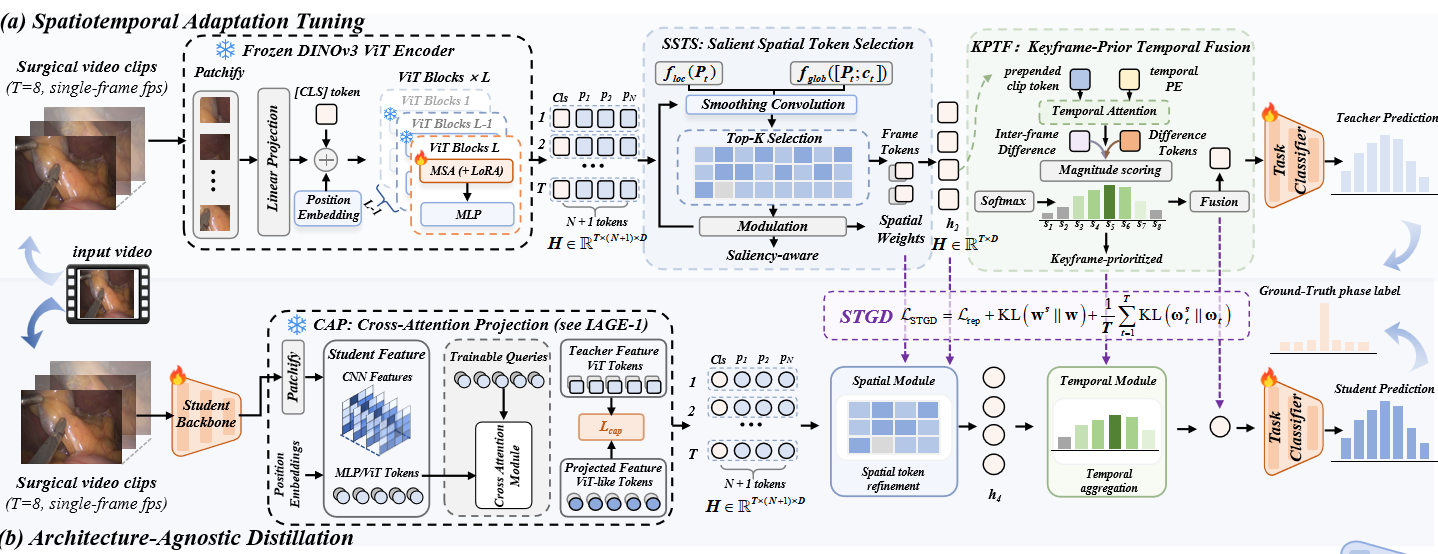
\includegraphics[width=\textwidth]{resources/method.png}
%     \caption{Visualization for our method.}
%     \label{fig:method}
% \end{figure*}


\section{Method}
\label{sec:method}

% Method overview / pipeline figure
\begin{figure*}[t]
    \centering
    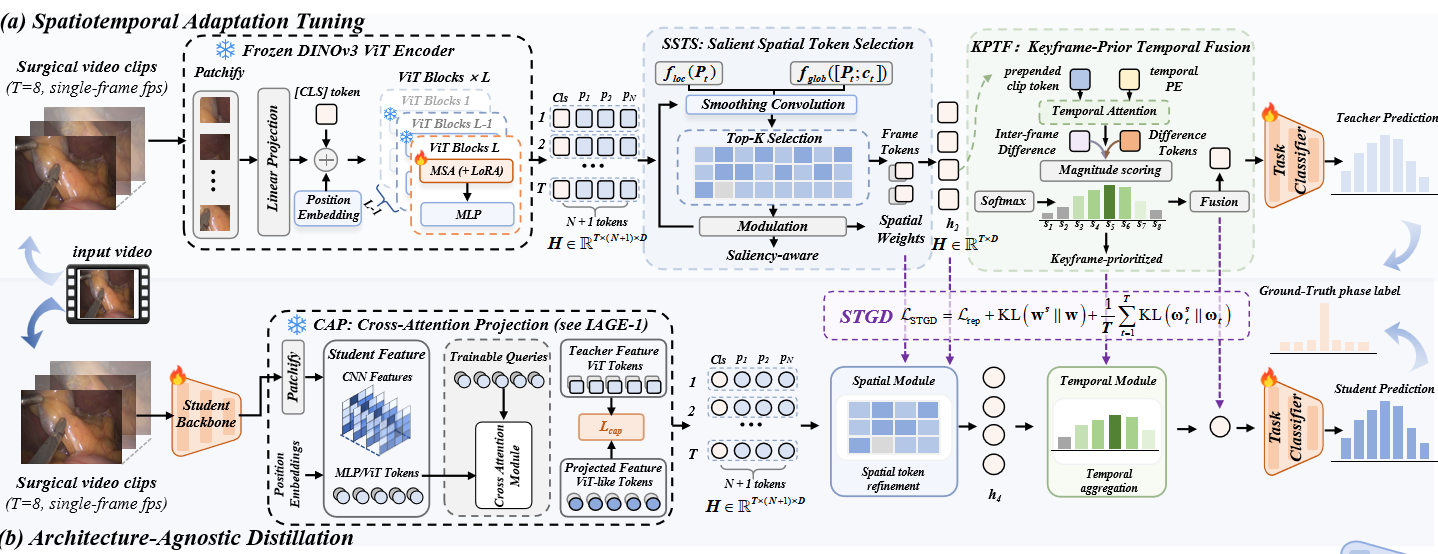
\includegraphics[width=\textwidth]{resources/method.png}
    \caption{Overview of the proposed framework. A frozen DINOv3 backbone is adapted to surgical video through a
    Salient Spatial Token Selection (SSTS) module and a Keyframe-Prior Temporal Fusion (KPTF)
    module, yielding SPR-Teacher. SPR-Lite further compresses the adapted model into lightweight backbones of
    arbitrary architectures via architecture-agnostic distillation.}
    \label{fig:method}
\end{figure*}



% ════════════════════════════════════════════════════════════════════
% TODO 图：整体 pipeline（视频适配 → 架构-无知蒸馏）
%   资源：figures/fig_pipeline.pdf（待制作）
% ════════════════════════════════════════════════════════════════════

\subsection{Overview}
\label{sec:method:overview}

% 写作要点（缩写 SSTS/KPTF/CAP/STGD 已在 intro 展开，本节不再重复给全称）：
% - 段 1：整体 roadmap——SPR-Teacher = DINOv3 + spatiotemporal 适配（SSTS 空间 + KPTF
%   时序），SPR-Lite = architecture-agnostic 蒸馏（CAP + STGD）。模块只用缩写带过，
%   不提 teacher/student 层级、参数/指标（放各自 subsection）。
%   2026-09-12 refine：全段改"动机在前"（few-shot 数据太少 → 借 DINOv3 泛化 → encoder
%   是 2D 无时序 → SSTS/KPTF → 资源受限 → 蒸馏 Lite），citation 上移到第一句。
% - 段 2（原 DINOv3 Backbone Review 并入本节）：只写后续模块依赖的形式化——input →
%   patchify → + 可学习 position embedding（覆盖 N+1 token）→ ViT block → per-frame
%   cls + patch tokens。不写死 B/14；预训练数据 LVD-1689M；LoRA/adaptation 归 §3.2。
%   2026-09-12 refine：过渡句改为"展开设计前先 review encoder 架构"；**删掉公式 (2)
%   （标准 ViT block 残差更新）及 MSA/LN/FFN 定义**——$\mathbf{E}$、$\mathbf{z}_{cls}$、
%   $\mathbf{z}^{(0)}$、$\mathbf{z}^{(\ell)}$、MSA/LN/FFN、$p$ 这些符号本节之后不再出现；
%   帧下标统一，直接给 $\mathbf{c}_t$、$\mathbf{P}_t$，因此 §3.2 开头与 §3.2.1 里
%   两处重复定义已删。

To overcome label scarcity in few-shot surgical phase recognition, we introduce \textsc{SPR-Teacher}, which adapts the generalization of a generic visual FM to the surgical domain.
As illustrated in Fig.~\ref{fig:method}, we first devise a spatiotemporal adaptation tuning that elevates independent frame-level features into sequence representations via SSTS and KPTF modules. By explicitly filtering the inherent redundancy of surgical videos to aggregate only the most discriminative spatiotemporal signals, this design imposes a strong inductive bias crucial for few-shot learning.
For resource-constrained clinical deployment, we further distill it, through architecture-agnostic distillation, into \textsc{SPR-Lite}, where CAP bridges representational gaps and STGD enriches sparse supervision with the teacher's priors.

% ════════════════════════════════════════════════════════════════════


% ════════════════════════════════════════════════════════════════════
\subsection{Spatiotemporal Adaptation Tuning}  % → SPR-Teacher (Phase 1 teacher)
\label{sec:method:video}

% 大纲（本节引入段 + 两个子模块 SSTS/KPTF + Adaptation Objective）：
% - 目标：让 frozen DINOv3 高效适配 surgical video domain（Phase 1 内不提蒸馏）。
% - 为什么只需轻量适配：DINOv3 已有强通用语义可直接泛化到 surgical domain，
%   只需围绕它做 spatiotemporal 适配，无需重训/大规模 FT（few-shot 下会过拟合）。
% - Surgical insight：手术视频 spatial + temporal 双重 redundancy——
%   spatial 上背景占多数像素但无判别信息；
%   temporal 上相位内稳态帧重复，关键信息集中在少数器械出现/转换帧。
% - 设计原则：用关键 spatial 区域 saliency prior + 关键 temporal 时刻 keyframe prior
%   注入 surgical 归纳偏置，以极小 trainable 参数撬动 frozen backbone。
% - → 落到两个模块 SSTS (§3.2.1) 和 KPTF (§3.2.2)。

Given a surgical video clip $\mathbf{X} \in \mathbb{R}^{T \times 3 \times H \times W}$ of $T$ consecutive frames, our goal is to predict the surgical phase of the last frame. To leverage the robust representation of FMs, we employ DINOv3 as the frame-level feature extractor. While we instantiate the framework with DINOv3, the adaptation operators below only assume a frozen image-level FM that emits per-frame tokens, so the framework does not hinge on a specific backbone. Specifically, for each frame $\mathbf{X}_t \in \mathbb{R}^{3 \times H \times W}$, DINOv3 splits the image into a regular grid of $N$ non-overlapping patches. Following linear projection and the prepending of a learnable class token $\mathbf{z}_{cls}$, the input sequence $\mathbf{z}^{(0)}$ is formulated as

\begin{equation}
  \mathbf{z}^{(0)} = [\,\mathbf{z}_{cls};\; \mathbf{E}\mathbf{x}_1;\; \cdots;\; \mathbf{E}\mathbf{x}_N\,]
  + \mathbf{E}_{pos}\in\mathbb{R}^{(N+1)\times D},
\end{equation}

\noindent where $\mathbf{E}$ is the projection matrix, $\mathbf{x}_i$ is the flattened $i$-th patch, and $\mathbf{E}_{pos}$ is the position embedding. After propagating through $L$ ViT blocks, DINOv3 outputs from its last layer:

\begin{equation}\mathbf{c}_t = \mathbf{z}_t^{(L)}[0], \qquad \mathbf{P}_t = \mathbf{z}_t^{(L)}[1{:}N].\end{equation}

\noindent where class token $\mathbf{c}_t$ summarizes the global context and spatial tokens $\mathbf{P}_t$ retain its spatial details for the frame. Consequently, the video clip $\mathbf{X}$ is initially encoded into a sequence of \textbf{frame-independent token sets} $(\mathbf{c}_{1:T}, \mathbf{P}_{1:T})$ lacking temporal interactions.
To establish spatiotemporal modeling, our adaptation progressively condenses these tokens into a compact representation.
Specifically, SSTS integrates spatial details $\mathbf{P}_t$ into $\mathbf{c}_t$ to produce \textbf{saliency-condensed frame tokens} $\tilde{\mathbf{c}}_{1:T} \in \mathbb{R}^{T \times D}$, which KPTF subsequently aggregates across time into a unified \textbf{clip-level feature} $\tilde{\mathbf{h}} \in \mathbb{R}^D$ for phase classification.



\subsubsection{Salient Spatial Token Selection}
\label{sec:method:video:spatial}

% ════════════════════════════════════════════════════════════════════
% SSTS 小节（v4：双视角打分 + 单选择损失）。整段替换 3_method.tex 里同名的
% \subsubsection 及其正文（含其后的 % 注释块）。
%
% 相对现正文的改动：
%   1) depthwise 3x3 卷积从"分数图平滑"改为"token 邻域精修"，位置移到两个视角之前；
%   2) 全局视角从单头点积注意力改为 f_glob([z_t; c_t])（与正文原意一致）；
%   3) 前向不再出现硬掩码，聚合就是按门加权平均，除以权重的总和；
%   4) f_mod 改成一次共享线性 value 投影 W_v，写成注意力的标准形式
%      （线性时"先投影再池化"与"先池化再投影"完全等价，代码里用的是后者）；
%   5) 新增唯一正则项 L_top-K：sigmoid 门对 top-K 选择集 S_t 的 BCE（不再显式写掩码）；
%   6) 删掉温度 τ、删掉"mask 后再除以 Σω 与 Σωω̄ 的双重归一化"、删掉
%      "We normalize the weights over the patches wherever they are used as a
%      distribution" 一句。
%
% 符号（全文约定，π 已废弃）：
%   ω̃_t ∈ R^N      打分
%   ω_t ∈ (0,1)^N  sigmoid 门，连续空间权重，也是蒸馏信号（STGD）
%   \mathbf{w}      时序侧权重（正体加粗，与 ω 区分）
%   \mathcal{S}_t   分数最高的 K 个 patch 的下标集合，L_top-K 直接用它分区
%   \hat{\mathbf{p}}_{t,i}  邻域精修后的 patch（原 patch 是 \mathbf{p}_{t,i}；
%                     \mathbf{z}_t 留给 backbone 的整体输出，本小节不使用）
%
% 落进正文后的两处配套（本文件不含）：
%   §3.3.2 STGD 信号列表统一成 \boldsymbol{\omega}^s_t / \boldsymbol{\omega}_t，
%     KL 写成 L_sp = (1/T)Σ_t KL(ω^s_t ‖ ω_t)；
%   §4.1 "the spatial hard mask keeps the top 30% of the N patches"
%     改成预算先验的说法（K = 0.3N 是先验，不是后处理的裁剪）。
% ════════════════════════════════════════════════════════════════════

Rather than treating all patch tokens equally, SSTS condenses the spatial tokens of a frame into its
frame token through a learned saliency gate that reinforces the informative regions.
Saliency in a surgical frame is spatially contiguous.
An instrument or a tissue spans a region rather than a single isolated patch.
Each patch should therefore be rated partly by its surroundings, and since a patch is only meaningful
in the frame's context, partly by the class token as well.
We restore the patch tokens to the $\sqrt{N}\times\sqrt{N}$ grid and score each on its own and with
the class token,
\begin{equation}
  \hat{\mathbf{P}}_t = \mathbf{P}_t + f_{\mathrm{dw}}(\mathbf{P}_t),
  \quad
  \tilde{\boldsymbol{\omega}}_t = f_{\mathrm{loc}}(\hat{\mathbf{P}}_t)
  + f_{\mathrm{glob}}([\hat{\mathbf{P}}_t;\,\mathbf{c}_t]).
  \label{eq:ssts-score}
\end{equation}

\noindent where $f_{\mathrm{dw}}$ is a depthwise $3\times3$ convolution over the reshaped patch grid,
and $f_{\mathrm{loc}}$ and $f_{\mathrm{glob}}$ are patch-shared MLPs.
The operator $[\cdot\,;\,\cdot]$ puts the class token next to every patch, and $\mathbf{p}_{t,i}$ and
$\hat{\mathbf{p}}_{t,i}$ denote the $i$-th token of $\mathbf{P}_t$ and $\hat{\mathbf{P}}_t$.
The score $\tilde{\boldsymbol{\omega}}_t \in \mathbb{R}^{N}$ holds one entry per patch, and the
refinement touches the patch tokens only, leaving the class token as the backbone produced it.
A sigmoid turns the scores into per-patch weights, which project the patches through a shared linear
$\mathbf{W}_v$ and pool them into the frame token,
\begin{equation}
  \boldsymbol{\omega}_t = \sigma(\tilde{\boldsymbol{\omega}}_t),
  \quad
  \tilde{\mathbf{c}}_t = \mathbf{c}_t
  + \alpha\,
  \frac{\sum_i \omega_{t,i}\,\mathbf{W}_v\,\mathbf{p}_{t,i}}{\sum_i \omega_{t,i}}.
  \label{eq:ssts-weight}
\end{equation}

\noindent With $\alpha$ a learnable scalar, the gate
$\boldsymbol{\omega}_t \in (0,1)^{N}$ a per-patch weight, and
$\tilde{\mathbf{c}}_t \in \mathbb{R}^{D}$ the saliency-condensed frame token.

In a surgical video the background occupies most of the field and the instrument or the tissue that
matters is a small share of the patches, so the gate should be sharpened to concentrate the frame
token on that share.
To this end we add a single training-time term built on a soft top-$K$ selection of the saliency
scores, which drives the gate up on the few patches that carry the content of the frame and down on
the background that does not.
Let $\mathcal{S}_t$ hold the indices of the $K$ largest entries of $\tilde{\boldsymbol{\omega}}_t$,
and the term be the cross-entropy of the gate against that selection,
\begin{equation}
  L_{\mathrm{top}\text{-}K} = -\frac{1}{N}\Big[\sum_{i \in \mathcal{S}_t}\log \omega_{t,i}
  + \sum_{i \notin \mathcal{S}_t}\log(1-\omega_{t,i})\Big].
  \label{eq:ssts-loss}
\end{equation}

\noindent The term pulls the gate towards the top-$K$ selection, and it is smallest once the two
agree.
Since a patch that stays in between is penalized whichever side of $\mathcal{S}_t$ it falls on,
agreement can only be reached by saturation, which sends the background towards $0$ and the selected
patches towards $1$ and turns the graded field of Eq.~\eqref{eq:ssts-weight} into a soft top-$K$.
SSTS scores each patch with its spatial neighborhood and the frame context, suppresses the background
through a soft top-$K$, and fuses the patches into the frame token.
% ────────────────────────────────────────────────────────────────────
\subsubsection{Keyframe-Prior Temporal Fusion}
\label{sec:method:video:temporal}

% Insight：跨帧上下文消歧 + 识别信息量更高的帧（而非均等对待 T 帧）。
%   注：是让 temporal pooling 给更 informative 的帧（器械操作明显、与邻帧差异大）更高权重。

% 设计（两路并行 + 融合）：
%   支路一 CLIP-token 时序聚合（主路径）：可学习 clip token h 拼到 c̃_{1:T} 前面（帧 token 加可学习时序 PE e_t），
%     过 temporal attention（TAttn，标准 MHA+FFN+LN 一个 block）→ 取 clip 位置输出为 clip summary ĥ。
%     一个算子搞定全局时序聚合（替代原 BiLSTM+conv+PE+CFA 四件套）。
%   支路二 关键帧打分（仿 STOP inter-frame temporal prompting，增强主路径）：对 SSTS 输出的 c̃_t 直接做帧间 delta
%     δ_t = c̃_t − c̃_{t-1} → depthwise 时序卷积 f_dw-1（1D，核 3）聚合差序列 → 分数 w̃_t = (1/D)‖f_dw-1(δ_{1:T})_t‖²
%     → softmax 权重 w（关键帧 = 帧间变化大的帧）→ 权重直接池化 c̃_t 出关键帧增强 token v = Σ_t w_t c̃_t（正文内联）。只读 c̃_t，与支路一并行。
%   融合：线性投影 f_fuse 拼接合并 ĥ 与 v（[ĥ; v] 过 Linear(2D→D)），输出 clip 特征 h̃。
% 正文顺序：先时序聚合 → 再关键帧打分 → 最后融合。两路都只读 c̃_t，真正并行。
% 注意（paper-idealized）：论文支路一是 CLIP-token attention、关键帧打分在 c̃_t 上（delta→conv→能量，仿 STOP）；
% 代码 dsx_bilstm 分支是 BiLSTM+conv+PE+CFA，_kts_scores/_predictor_lg_scores 在 fused_t（CFA 后）上、MLP+0.1×局部-全局。
%

% 关键公式（$\tilde{\mathbf{c}}_{1:T}$ 为 §3.2.1 的 saliency-condensed frame tokens；正文公式顺序 = 支路一时序聚合 → 支路二关键帧打分 → 融合）：
%   支路一：$\hat{\mathbf{h}} = \mathrm{TAttn}([\mathbf{h}, \tilde{\mathbf{c}}_1+\mathbf{e}_1, \tilde{\mathbf{c}}_2+\mathbf{e}_2, \ldots, \tilde{\mathbf{c}}_T+\mathbf{e}_T])[0]$，
%     可学习 clip token h 聚合跨帧上下文，clip 位置输出即 clip summary ĥ（D 维）。
%   支路二：$\boldsymbol{\delta}_t = \tilde{\mathbf{c}}_t - \tilde{\mathbf{c}}_{t-1}$ 为帧间变化（inter-frame delta）。
%     $\tilde{\mathbf{w}}_t = \tfrac{1}{D}\|f_{\mathrm{dw}\text{-}1}(\boldsymbol{\delta}_{1:T})_t\|^2$ 为每帧 pre-softmax 分数（能量），
%     $\mathbf{w} = \mathrm{softmax}(\tilde{\mathbf{w}}_{1:T})$ 为关键帧权重，
%     $\mathbf{v} = \textstyle\sum_t w_t \tilde{\mathbf{c}}_t$ 为 keyframe-pooled token（正文内联）。δ 公式已移入正文（不占公式行）。
%   融合：$\tilde{\mathbf{h}} = f_{\mathrm{fuse}}([\hat{\mathbf{h}}; \mathbf{v}])$ 线性投影合并两路（[ĥ; v] concat 后 Linear(2D→D)），无门控。

%   输入
%
%   每帧 SSTS 输出的 saliency-condensed frame token，按时间顺序排成序列，形状 T × D（T 帧，每帧一个 D 维向量），
%   这是 KPTF 唯一的输入。
%
%   支路一：CLIP-token 时序聚合（temporal attention）
%
%   - 结构：可学习 clip token h（D 维）拼在序列最前面，序列变成 (T+1) × D；
%     帧 token 先加可学习时序位置编码 e_t（每帧位置 t 一个 D 维向量），标记帧顺序
%     （attention 排列不变，必须显式给顺序——这一点和 BiLSTM 相反，BiLSTM 自带顺序感）。
%   - 主体：temporal attention（TAttn）= 标准 MHA + FFN + LayerNorm 的一个 transformer block，
%     在 (T+1) 个 token 上做自注意力，每帧都能聚合整段 clip 的上下文，clip token 汇总全局时序信息。
%   - 输出：取 clip 位置输出（[0]，D 维）当 clip summary ĥ，作为整段摘要。
%   - 副产品：注意力矩阵 (T+1) × (T+1)（可视化）。
%
%   支路二：关键帧打分（帧间变化 delta，仿 STOP inter-frame temporal prompting）
%
%   - 输入：SSTS 输出的 c̃_t（形状 T × D，KPTF 原始输入），与支路一并行、互不依赖。
%   - 关键观察：剧烈动作的帧与上一帧差异最大，这类帧信息量最高（仿 STOP §3.4 的 Δh^s）。
%   - 帧间差：δ_t = c̃_t − c̃_{t-1}；第一帧与自身比（差为 0）。
%   - 聚合：depthwise 时序卷积 f_dw-1（1D，核 3；§3.2.1 的 f_dw 是 2D 版）聚合差序列，压掉单帧噪声（仿 STOP eq9 的 N_t）。
%   - 分数：w̃_t = (1/D)‖f_dw-1(δ_{1:T})_t‖²，每帧 pre-softmax 分数的均方模长（仿 STOP eq10 的 L2 池化）；
%     saliency 已通过 c̃_t 继承（SSTS 加权聚合 patch），变化反映判别区域而非背景（仿 STOP 的 1+βr 加权）。
%   - 权重：w = softmax(w̃_{1:T})，和为 1（变化大的帧权重高）。δ 公式直接写在正文（不占公式行）。
%   - 加权池化：权重 w 直接加权求和帧 token（Σ_t w_t c̃_t）→ 关键帧增强 token v（正文内联）。
%   - 代码差异（paper-idealized）：代码 _kts_scores/_predictor_lg_scores 在 fused_t（CFA 后）上、MLP+0.1×局部-全局 打分；
%     论文简化为 c̃_t 上的 delta→conv→能量 打分（仿 STOP），代码保持现状。
%
%   两路融合：线性投影 f_fuse 拼接合并 temporal token ĥ（支路一 eq8）与关键帧增强 token v（支路二，正文内联）
%
%   - 线性投影：拼接 [ĥ; v]（2D 维）过 Linear(2D→D) 一次投影出 clip 特征 h̃，无门控、无残差插值。
%
%   输出
%
%   - h̃：形状 D，融合后的 clip 特征，送分类头。
%   - w：形状 T，每帧时间权重（蒸馏信号 + 可解释）。
%   - 注意力矩阵：(T+1) × (T+1)（clip token + T 帧，可视化）。

The saliency-condensed frame tokens stay isolated between frames, so KPTF carries out the temporal modeling
that fuses the sequence into a clip-level feature.
A learnable clip token $\mathbf{h}$ is prepended to the sequence and lets every frame gather
cross-frame context through temporal attention, whose output at the clip position is the clip summary
$\hat{\mathbf{h}}$,
\begin{equation}
  \hat{\mathbf{h}} = \mathrm{TAttn}\!\big([\mathbf{h}, \tilde{\mathbf{c}}_1+\mathbf{e}_1, \tilde{\mathbf{c}}_2+\mathbf{e}_2, \ldots, \tilde{\mathbf{c}}_T+\mathbf{e}_T]\big)[0].
\end{equation}

\noindent where $\mathrm{TAttn}$ is a transformer block over the $T+1$ tokens of the augmented
sequence, and $\mathbf{e}_t$ a learnable temporal positional encoding that keeps the frame order.

Surgical video is temporally redundant, as the field holds a steady state through most of a phase, and
the frames that differ markedly from their neighbors carry the discriminative evidence.
The keyframe-scoring branch, inspired by inter-frame temporal prompting~\cite{liu2025stop},
rates each frame by its inter-frame difference
$\boldsymbol{\delta}_t = \tilde{\mathbf{c}}_t - \tilde{\mathbf{c}}_{t-1}$ (with
$\boldsymbol{\delta}_1=\mathbf{0}$), so that a frame of marked
change outranks one that holds steady.
A one-dimensional depthwise convolution $f_{\mathrm{dw}\text{-}1}$ of kernel size $3$ aggregates the
difference sequence, whose mean squared magnitude gives the per-frame score $\tilde{\mathbf{w}}_t$.
Softmax turns the scores into the frame weights $\mathbf{w}$,
\begin{equation}
  \tilde{\mathbf{w}}_t = \tfrac{1}{D}\big\| f_{\mathrm{dw}\text{-}1}(\boldsymbol{\delta}_{1:T})_t \big\|^{2}, \qquad
  \mathbf{w} = \mathrm{softmax}(\tilde{\mathbf{w}}_{1:T}).
\end{equation}

\noindent The weights quantify how much each frame contributes to the clip and pool the sequence into
a keyframe-pooled token $\mathbf{v} = \textstyle\sum_{t}w_{t}\tilde{\mathbf{c}}_{t}$.
The clip summary and the keyframe-pooled token carry complementary evidence, the context of the whole
clip and the motion of its most informative frames, so a fusion operator $f_{\mathrm{fuse}}$ merges
them,
\begin{equation}
  \tilde{\mathbf{h}} = f_{\mathrm{fuse}}\!\big([\hat{\mathbf{h}};\, \mathbf{v}]\big).
\end{equation}

KPTF fuses the clip summary and the keyframes into the clip-level feature $\tilde{\mathbf{h}}$, which
captures the informative motions and yields a more accurate phase prediction.

% ────────────────────────────────────────────────────────────────────
\subsubsection{Adaptation Objective}
\label{sec:method:video:loss}

% 写作要点：
%
% 可训练参数（DINOv3 backbone 绝大部分层冻结，仅最后 block 的 Q/V 加 LoRA，以保留通用语义）：
%   - LoRA adapters：加在最后 transformer block 的 Q/V projection（~0.4M），做 task
%     adaptation 而不破坏预训练特征空间；
%   - 两个适配模块 SSTS + KPTF（随机初始化）；
%   - Classification head（LN + Linear）。
%   backbone 主体冻结，仅以上适配部分 + head 可训练。
%
% Loss：$L_\mathrm{tuning} = L_\mathrm{CE} + L_{\mathrm{top}\text{-}K}$（2026-09-23 起
%   SSTS 的选择项计入 tuning 目标，不再是单一 CE）。
%   $\hat{\mathbf{y}} = f_\mathrm{cls}(\tilde{\mathbf{h}})$，$\tilde{\mathbf{h}}$ 来自 KPTF；
%   $L_{\mathrm{top}\text{-}K}$ 是 §3.2.1 的 sigmoid 门选择项，只正则化空间门控、不改前向。
%   符号体例：全文 loss 用正体 $L$（SSTS 里的 $\mathcal{L}_{\mathrm{top}\text{-}K}$ 已改成
%   $L_{\mathrm{top}\text{-}K}$），与 §3.3.2 的 $L_\mathrm{rep}$、$L_\mathrm{stgd}$ 统一。

The DINOv3 backbone stays largely frozen to preserve its general pretrained semantics. Only a
small set of parameters is trained, the LoRA adapters~\cite{hu2022lora} on the query/value projections of the
last ViT block, the two adaptation modules SSTS and KPTF, and a linear classification head
$f_{\mathrm{cls}}$.
Training minimizes the phase cross-entropy together with the top-$K$ selection term of SSTS,
\begin{equation}
  \hat{\mathbf{y}} = f_{\mathrm{cls}}(\tilde{\mathbf{h}}), \qquad
  L_\mathrm{tuning} = L_\mathrm{CE} + L_{\mathrm{top}\text{-}K}.
\end{equation}

% ════════════════════════════════════════════════════════════════════
\subsection{Architecture-Agnostic Distillation}  % → SPR-Lite (Phase 2 student)
\label{sec:method:distill}

% 引入（承上启下 + 架构依赖问题 + 三大家族 + 两个设计模块，均不写具体数字）：
% - 承上启下：SPR-Teacher 做 spatiotemporal 适配后继承了 DINOv3 的泛化、few-shot 表现好，
%   但仍是 architecture-dependent（绑死 DINOv3 ViT 形态）。
% - 架构依赖的缺点：部署端灵活度不足、参数量大加载缓慢、推理效率低。
% - 因此引入 architecture-agnostic 蒸馏 → SPR-Lite：可蒸馏到任意架构轻量 student，
%   达到部署友好 + 实时推理。
% - **2026-09-14 用户重构**：三大家族（CNN / ViT / hybrid）的铺陈**从 §3.3.1 上移到本段**，
%   顺序是：主流轻量模型就这三家 → ViT 天然与 teacher 同形、不需要接口 → 问题集中在
%   非 ViT 的 feature map（cell 数与宽度都对不上 teacher patch），teacher 的 prior 直接
%   用不上 → 所以 CAP 就为解决这一处不一致而生 → 由此才谈得上 architecture-agnostic。
%   §3.3.1 因此只剩"以 CNN 为代表 → CAP → 同形 token → SSTS^s / KPTF^s 跑出 ŷ^s"。
% - 两个设计模块：
%   (1) CAP 跨架构表征投影：bridge ViT teacher 与不同架构 student 的表征差距，
%       使蒸馏对 student 架构无关；
%   (2) STGD 时空引导蒸馏：few-shot 下蒸馏信号 scarce，用 SPR-Teacher 的 spatial/temporal
%       prior 引导 student，提升蒸馏效率。

SPR-Teacher inherits the generalization of DINOv3 and delivers promising few-shot
performance, but it remains tied to the heavy ViT architecture, which restricts deployment
flexibility and slows both loading and inference.
We therefore distill it into \textsc{SPR-Lite}, whose backbone can follow any mainstream
lightweight architecture.
Those architectures fall into three families: CNN, ViT, and hybrid.
A ViT student already emits a class token and patch tokens in the teacher's form, whereas the other
two architectures emit feature maps whose spatial cells might not match the teacher's tokens,
so the teacher's spatial and temporal priors cannot be applied to them directly.
CAP resolves this at the last stage of the student, transforming the feature map into the teacher's
token space so that the student carries the same per-frame tokens as the teacher.
The student then employs SSTS and KPTF of the same structure, which is what makes the scheme
architecture-agnostic.
STGD compensates for the scarce supervision of the few-shot regime with the teacher's
spatiotemporal priors.

% ────────────────────────────────────────────────────────────────────
\subsubsection{Student Architecture}
\label{sec:method:distill:student}

% 大纲（以 CNN 为代表 → CAP 前置 → SSTS/KPTF 原样复用）：
% - **2026-09-14 用户重构**：三大家族（CNN / ViT / hybrid）的论述已上移到 §3.3 引入段，
%   本小节不再重复，只一句"以 CNN 为代表例"承接。
% - **2026-09-14 重构（用户定）**：CAP 从"旁路对齐损失"前移为 student 的前端。
%   student 只暴露 last stage 特征图 $\mathbf{M}_t$ → CAP 投进 teacher token 空间
%   → 得到与 teacher 同形态的 (class token, patch tokens) → SSTS / KPTF **定义原样复用**。
%   因此本小节删掉了原先那套独立的特征图版定义（格点当 patch、加权池化公式、以及
%   C→D linear adapter），只剩一段讲接口。注意 $^s$ 只是归属标记（见下），**不是**
%   student 专属变体。
%   收益：① 正文少一套平行定义；② STGD 的 $\mathrm{KL}(\boldsymbol{\omega}^{s}_t\|\boldsymbol{\omega}_t)$
%   不再需要"把 h×w 双线性 resize 到 N"这个正文不写的隐藏操作（两者现在都是长度 N）。
%   代价：CAP 的 patch query 必须带位置编码做软空间锚定（见 §3.3.2），否则 student 的 patch token
%   没有空间语义，SSTS 的网格平滑/top-K 与上面那条 KL 都站不住。
% - 上下标规范：下标 = 序列索引（帧 $t$、patch $i$）；层号用括号上标 $(\ell)$（仅 §3.1 用）；
%   上标 = 变体/标签（student $s$、loc/glob）；saliency 用波浪号 $\tilde{}$；位置选择用方括号 $[0]$/$[1{:}N]$。
%   空间/时间权重用两个不同基符号区分（$\boldsymbol{\omega}_t$=spatial、$\mathbf{w}$=temporal），不占上标槽位。
%   teacher 不标（默认模型）；
%   student **输出**一律上标 $s$（$\tilde{\mathbf{c}}^{s}_t$、$\tilde{\mathbf{h}}^{s}$、
%   $\boldsymbol{\omega}^{s}_t$、$\mathbf{w}^{s}$），否则两份实例分不开；
%   但 **SSTS / KPTF 算子本身不标 $^s$**——重构后 student 用的是同一定义（两份实例、
%   结构相同但**不共享权重**），不存在 student 专属变体。
%   指代 student 那一份时用**属格**："the student's SSTS and KPTF"（§3.3.1）或
%   "of the same structure"（§3.3 引入段），不要写成 $\mathrm{SSTS}^s$ 这种把上标挂在
%   模块名上的写法（2026-09-14 用户否掉了两版：先标 $^s$、后写 "run with the teacher's
%   definitions"，都不行）。
% - 四个蒸馏信号（$\boldsymbol{\omega}_t$、$\mathbf{w}$、$\tilde{\mathbf{c}}_t$、$\tilde{\mathbf{h}}$）及其
%   student 对应（上标 $s$）由 §3.3.2 引入，本节只讲 student 怎么接上，不重复枚举。
%

We take CNN as the representative student.
It is image-based and exposes a last-stage feature map
$\mathbf{M}_t\in\mathbb{R}^{C\times h\times w}$, which CAP maps into the teacher's token space,
producing a class token $\mathbf{c}^{s}_t$ and $N$ patch tokens $\mathbf{P}^{s}_t$ of width $D$.
The student therefore yields tokens of the same form as the teacher, which its SSTS and KPTF
aggregate progressively into the saliency-condensed frame tokens $\tilde{\mathbf{c}}^{s}_{1:T}$ and then
the clip-level feature $\tilde{\mathbf{h}}^{s}$, from which the classification head gives the clip
prediction $\hat{\mathbf{y}}^{s}$.

% ────────────────────────────────────────────────────────────────────
\subsubsection{Distillation Scheme}
\label{sec:method:distill:scheme}

% 大纲（异构→CAP、稀疏→STGD + 总 loss；训练配方 → §4）：
% 开篇（简洁）：直接讲异构 challenge——teacher 与 student 表征空间不同、语义单元不匹配，
%   特征无法直接比较 → 由 CAP 解决（稀疏 motivation 放到后面 STGD 段才说）。
%   开篇顺带交代来源 ScaleKD (Fan et al., CVPR'24)，正文 CAP 段不再提（paper-idealized，代码无此模块）。
%
% ─── 线 1: CAP（Cross-Attention Projection，feature-level）───
% **定位（2026-09-14 重构后）**：CAP 不再是"旁路对齐损失"，而是 **student 的前端/接口层**——
%   它把 student 的 last stage 特征图变成 teacher 形态的 (class token, patch tokens)，
%   此后的 SSTS / KPTF 原样复用（见 §3.3.1）。L_cap 仍是那个 ℓ2 对齐项，用来拉住这个接口
%   别漂离 teacher 的 token 空间。
% 动机：异构。CAP 作用于最后一个 stage（正文第一句给正面理由：该 layer 任务适配最强、
%   与 teacher 的异构差异最大；不再用"只开放最后一层微调"作因果解释）。
%   （措辞：last stage 是"任务相关性最强"，不说"被任务适配的那层"——student 整个 backbone 都在训。）
%   teacher 最后一层输出 per-frame class token $\mathbf{c}_t$ + patch tokens $\mathbf{P}_t$；
%   student 最后一层输出特征图 $\mathbf{M}_t$，语义单元（patch vs grid cell）与维度（D vs C）都不同。
%   **对齐机制 v3（2026-09-12 用户定稿：回退到 attention 版，正文必须讲清 N/D 怎么对齐）**：
%   两步：
%   (i) patchify（解决**维度** C→D）：把 $\mathbf{M}_t$ 的 $h\times w$ 个 cell 摊平成 $h w$ 个
%       spatial token，每个过共享线性映射 $C\to D$，加位置编码保留网格布局；
%       此时 token 数仍是 $h w$，**还没**解决计数。
%   (ii) cross-attention（解决**计数** $h w\to N$，且不需要任何 resize）：query 侧 =
%       $N$ 个可训练 patch query + 1 个可训练 class query（全 D 维），student token 作 K/V。
%       **输出长度由 query 数决定、与 K/V 长度无关**——每个 query 经 softmax 把整条 $h w$ 序列
%       加权聚合成 1 个 D 维向量，故得 $N+1$ 个输出；输出宽度 = query 宽度 = $D$。
%   (iii) 拆分：class query 输出 = $\mathbf{c}^s_t$，$N$ 个 patch query 输出 = $\mathbf{P}^s_t$。
%   **cls 学生侧显式得到（用户明确要求写清）**：student（CNN）结构上无 cls，正文必须点明
%   $\mathbf{c}^s_t$ 来自**专门的 class query 槽位**、与 patch query 同构、input-dependent，
%   而不是对特征图做 pooling 的摘要。
%   **代价（知情接受）**：$N+1$ 个 query 对 $h w$ 个 key，softmax 权重被稀释、收敛慢。
%   **2026-09-14 补丁（CAP 前置重构带出）**：原先 query↔cell 的空间对应"只由位置编码 + L2
%   隐式引导，几何上不保证"。当时 CAP 只喂 $L_\mathrm{cap}$，这个不确定性只影响一个损失项；
%   现在 CAP 前置到任务路径，SSTS 的 3×3 网格平滑、top-K 选区域、以及
%   $\mathrm{KL}(\boldsymbol{\omega}^{s}_t\|\boldsymbol{\omega}_t)$ 全都假设 student 的 patch token
%   **有空间语义**，所以必须补锚定 → 给 **patch query 侧**加位置编码，使 query 对其对应空间
%   区域的 cell 响应最强（正文已落一句）。cls query 不带位置（cls 本就无空间位置）。
%   这是为保 ScaleKD 谱系付的代价；v2 的插值版（h×w 重采样到 14×14）能天然解决，
%   但放弃了 ScaleKD 的说法，用户 2026-09-14 选择保留谱系 + 加锚定。
%   **与 ScaleKD 的关系**：此步完整对应 ScaleKD modification (iii)（可训练 query、共享 teacher
%   分辨率的 cross-attn 聚合），"Inspired by ScaleKD" 成立。
%   **与 ScaleKD 的差别（保留）**：ScaleKD 的 proj_student 是 3×3 Conv+BN+ReLU 保 C 维
%   （fmd.py:154），C→D 藏在 cross-attn 的 K/V 投影里（attention.py:214-215）；我们正文写成
%   显式的共享线性映射，读者更好懂。
%   **行文口径（2026-09-12 用户定）**：CAP 段只讲"特征图怎么变成 tokens"，讲完直接给 L2 对齐
%   公式即可——不要铺陈"不需要 resize""不假设网格已重合"这类辩护性内容，也不要给 class query
%   写"而非 pooling 摘要"的对比，一句"显式产出 $\mathbf{c}^s_t$"够。开篇三句压成两句
%   （teacher 一行 / student 一行对比），长句拆短，$h\times w$ 用 $\times$ 不用 $\,w$。
%   **补充（同日）**：不用口语 + 不用冒号句式（禁"The dimension now matches, but the count does not:"）；
%   **别整段按 $N$/$D$ 两个符号叙事**，要对着实体讲（"student token 与 teacher patch token 同宽"
%   "聚合出的 patch token 数与 teacher 一样多"），符号只在首次定义处出现；**公式只写一条**——
%   patch 与 cls 不再拆成两个 $\ell_2$ 项，直接一条 norm 比较整体 token：
%   $\|[\mathbf{c}_t;\mathbf{P}_t] - \mathrm{CAP}(\mathbf{M}_t;\mathbf{q}_\mathrm{cls},\mathbf{q}_{1:N})\|_2^2$。
%   **cls 补丁（2026-09-12 定）**：student（CNN）结构上无 cls，而 DINOv3 teacher 的 cls 是 SSTS/KPTF
%   的主角，所以给 CAP 补 1 个可训练 class query（attend $N$ 个 patch token → input-dependent 全局 token），
%   与 teacher 原始 $\mathbf{c}_t$ 对齐。**与 ScaleKD 的差别**：ScaleKD 两边都切掉 cls
%   （vit.py `_format_mid_feat` / `out_type='featmap'` 都做 `x[:, num_extra_tokens:]`；ViT student
%   config 显式 `with_cls_token=False`），cls 只走 logit KD；我们额外在特征层对齐 cls。
%   **已知重叠（用户已知并接受）**：STGD 的 $L_\mathrm{rep}$ 已对齐 $\tilde{\mathbf{c}}^s_t \leftrightarrow \tilde{\mathbf{c}}_t$
%   （$\tilde{\mathbf{c}}_t = \mathbf{c}_t + \alpha f_\mathrm{mod}$），与 CAP 的
%   $\mathbf{c}^s_t \leftrightarrow \mathbf{c}_t$ 高度相关；选择保留两者，STGD 不动。
%   符号区分：CAP 对齐**原始** $\mathbf{c}_t$（无波浪线），STGD 对齐**调制后** $\tilde{\mathbf{c}}_t$。
%   对齐：单条 squared ℓ2 比较整体 token（patch 与 cls 不拆成两项）。
% 公式（当前版）：
%   $L_\mathrm{cap} = \frac{1}{T}\sum_t \big\|[\mathbf{c}_t; \mathbf{P}_t]
%     - \mathrm{CAP}(\mathbf{M}_t; \mathbf{q}_\mathrm{cls}, \mathbf{q}_{1:N})\big\|_2^2$。
%   同一 projector 走所有 student 家族 → architecture-agnostic；
%   弥合 CNN/Hybrid 异构，near-homogeneous ViT student 不受影响。
%
% ─── 线 2: STGD（时空引导蒸馏，承载全部中间信号）───
% 承上启下：CAP 对齐特征空间之后，STGD 解决 few-shot 蒸馏信号稀疏的问题。
% 动机：稀疏。标签太少 → 用 SPR-Teacher 的 4 个 spatiotemporal 中间信号去弥补，
%   末尾再补常规的 logit 项（不再提 "logit-only KD 太稀疏" 的旧框架）。
% 正式引入 4 个中间信号（一句，不用 "Two are..." 口语化）：
%   表征类：saliency-condensed frame tokens $\tilde{\mathbf{c}}_{1:T}$ + clip-level feature
%     $\tilde{\mathbf{h}}$；先验类：spatial weights $\boldsymbol{\omega}_{1:T}$ + temporal weights
%     $\mathbf{w}$。
% 对齐（一句）：先列出 student 的 4 个符号 c̃^s_{1:T}、h̃^s、ω^s_{1:T}、w^s（"student 也有这几个"），
%   再统一对齐——表征类 cosine、先验类 KL。
% **2026-09-12 用户 review 后的修正（已落到正文）**：
%   (1) 学生侧 h̃^s 原先无出处（§3.3.1 只列了 w^s 和 ŷ^s）→ 已在 §3.3.1 补 "the clip
%       representation $\tilde{\mathbf{h}}^{s}$"；
%   (2) ŷ 层级含混：teacher 只有 clip 预测（§3.2.3 单一 CE），曾为 L_dec 的双 level 蒸馏补过
%       per-frame 预测 $\hat{\mathbf{y}}_{1:T}$；**2026-09-12 用户决定 L_dec 整项删掉**（公式与解释句
%       全删），per-frame 预测因此在正文失去用途 → §3.2.3 的 per-frame 句、§3.3.1 学生侧
%       $\hat{\mathbf{y}}^{s}_{1:T}$ 一并删除，全篇只剩 clip 预测 $\hat{\mathbf{y}}$ / $\hat{\mathbf{y}}^{s}$。
%       注意：代码里 per-frame logit KD（train_distill_final.py 的 per_frame_logits + kd_loss）仍在，
%       属 paper-idealized（论文不写、代码保留）。
%   (3) KL 原来写成 $\mathrm{KL}(p, q)$ 且无方向 → 改 $\mathrm{KL}(p \,\|\, q)$，student 作 P；
%       "each per-patch weight map" 的 each 不成立（w 已是 softmax 分布、帧数相同）→ 正文分开讲，
%       并交代 resize→normalize 的先后；
%   (4) 公式前那句把公式复述了一遍 → 压成"we group the representation terms as L_rep…"，
%       L_rep 符号得以引入；公式末尾句号删掉再接 where；
%   (5) ~~$L_\mathrm{dec}$ 加 per-frame 项~~ → **2026-09-12 用户改：$L_\mathrm{dec}$ 整项不写**；
%   (6) 与 CAP 段的一致性：**2026-09-14 CAP 前置重构后此项已消解**——原先 student 的
%       $\boldsymbol{\omega}^{s}_t$ 落在 $h\times w$ 网格、与 teacher 的 $\boldsymbol{\omega}_t$（长度 N）
%       不同，KL 实际靠双线性 resize（distill_modules_final.py:95-101）强行对齐，而正文按用户
%       2026-09-12 的指示"resize/normalize 这类操作细节一个字都不写"，等于把这一步藏起来了。
%       现在 CAP 前置产出 N 个 patch token，$\boldsymbol{\omega}^{s}_t$ 与 $\boldsymbol{\omega}_t$
%       都是原生长度 N，**公式自己成立，不需要任何 resize**。STGD 段落行文体例不变：只讲**理由**
%       （prior 信号记录 teacher 在哪/何时看，是 few-shot 标签给不了的监督）**+ 加入蒸馏目标**；
%   (7) 命名统一：$\tilde{\mathbf{c}}_t$ 三处叫法（frame representation / class token / frame
%       tokens）统一；$\mathbf{v}$ 原叫 keyframe-enhanced token、
%       与 $\tilde{\mathbf{h}}$ 的 keyframe-enhanced clip token 撞名 → $\mathbf{v}$ 改叫
%       **keyframe-pooled token**。
%   (8) **2026-09-23 命名总表（§3.2 引入段给定，全篇按此用，不加粗）**：
%       $(\mathbf{c}_t, \mathbf{P}_t)$ = frame-independent token sets；
%       $\tilde{\mathbf{c}}_t$ = saliency-condensed frame tokens（旧的 saliency-aware 一律改掉）；
%       $\tilde{\mathbf{h}}$ = clip-level feature（旧的 clip feature / keyframe-enhanced clip
%       token 一律改掉）；$\mathbf{v}$ = keyframe-pooled token。§3.2.2 与 §3.3.1/§3.3.2 已同步。
% 公式（当前版，一个方程两行：L_rep / L_stgd）：
%   $L_\mathrm{rep} = d_{\cos}(\tilde{\mathbf{h}}^{s}, \tilde{\mathbf{h}})
%     + \frac{1}{T}\sum_t d_{\cos}(\tilde{\mathbf{c}}^{s}_t, \tilde{\mathbf{c}}_t)$
%     （2026-09-12 用户定版：**公式里只出现 $d_{\cos}$，不再展开 $1-\cos$**；正文只留一句
%      "where $d_{\cos}$ is the cosine distance between two tokens" + 一句解释（按方向比、对尺度不敏感），
%      **不写符号定义公式**。符号名不用 $\mathrm{sim}$（用户嫌丑），也不用 $\cos(\cdot,\cdot)$ 两参写法。
%      注意：$d_{\cos}$ 定义里含 $1-\cos$，所以正文说 "distance" 而非 "similarity"，
%      避免与"最小化相似度"读起来矛盾；好处 $L_\mathrm{rep}\ge 0$、$L_\mathrm{stgd}$ 恒非负）
%   $L_\mathrm{stgd} = L_\mathrm{rep}
%     + \mathrm{KL}(\mathbf{w}^{s} \| \mathbf{w})
%     + \frac{1}{T}\sum_t \mathrm{KL}(\boldsymbol{\omega}^{s}_t \| \boldsymbol{\omega}_t)$
%     （2026-09-12 用户定版：**带 $\sum$ 的项排最后**，非连加项在前）
%
% ─── 总 loss ───
% $L = L_\mathrm{tuning} + L_\mathrm{cap} + L_\mathrm{stgd}$（λ 全默认 1）。
%   2026-09-23：$L_\mathrm{CE}$ → $L_\mathrm{tuning}$，与 §3.2.4 的目标对齐
%   （$L_\mathrm{tuning} = L_\mathrm{CE} + L_{\mathrm{top}\text{-}K}$）——
%   student 复用同结构 SSTS/KPTF，因此也带 top-K 选择项。
% 训练配方（优化器 / schedule / 增强 / EMA 等）统一放 §4 Implementation Details。

% TODO 图：模块级架构图（CAP / STGD 各一张）
\noindent\textbf{Cross-Attention Projection (CAP).}
CAP is the front end of the student pipeline, converting the feature map into the token form that
every later module takes as input.
Its design follows ScaleKD~\cite{fan2024scalekd} and is built as a cross-attention interface.
The last stage holds the most task-specific representation, so CAP converts the feature map there.
It flattens $\mathbf{M}_t$ into $h\times w$ spatial tokens and maps each token from $C$ to the
teacher's width $D$ with a shared linear projection, adding positional embeddings that keep the grid
layout.
Each student token then has the teacher's width, so only their number remains to reconcile.
CAP resolves the count mismatch on the query side.
It keeps a set of learnable queries in the teacher's space, one per teacher token:
a patch query for each of the teacher's patches, plus a single class query for the
class slot the student lacks.
Cross-attention emits one output per query, so the output length is decided by the queries rather
than by the feature map.
The $h\times w$ cells are therefore aggregated into exactly as many patch tokens $\mathbf{P}^{s}_t$
as the teacher has.
Each patch query carries the position of the teacher patch it stands for, so a query draws most
strongly on the student cells occupying the same region of the frame.
The student's patch tokens thus keep a spatial layout, which the grid operations of SSTS rely on,
and the class query produces the student's class token $\mathbf{c}^{s}_t$.
A squared $\ell_2$ distance then aligns the student tokens with the teacher's,
\begin{equation}
  L_\mathrm{cap} = \frac{1}{T}\sum_{t=1}^{T}
  \big\|\,\big[\mathbf{c}_t;\,\mathbf{P}_t\big]
  - \mathrm{CAP}\big(\mathbf{M}_t;\, \mathbf{q}_\mathrm{cls}, \mathbf{q}_{1:N}\big)\,\big\|_2^2 .
\end{equation}

\noindent\textbf{Spatiotemporally-Guided Distillation (STGD).}
To address the sparsity of few-shot supervision,
STGD distills the teacher's spatiotemporal knowledge through
four intermediate signals.
The representation signals are the saliency-condensed frame tokens
$\tilde{\mathbf{c}}_{1:T}\in\mathbb{R}^{T\times D}$ and the clip-level feature
$\tilde{\mathbf{h}}\in\mathbb{R}^{D}$, while the prior signals are the spatial gates
$\boldsymbol{\omega}_{1:T}\in\mathbb{R}^{T\times N}$ and the temporal weights
$\mathbf{w}\in\mathbb{R}^{T}$.
The temporal weights $\mathbf{w}$ form a distribution over frames, and the
spatial gates $\boldsymbol{\omega}_{t}$ are normalized over the patches, so
each enters the KL as a distribution.
The prior signals encode where and when the teacher attends, information that the scarce labels do
not provide.
The student pipeline exposes the same four signals
$\tilde{\mathbf{c}}^{s}_{1:T}$, $\tilde{\mathbf{h}}^{s}$, $\boldsymbol{\omega}^{s}_{1:T}$, and
$\mathbf{w}^{s}$, and aligns each to the teacher's counterpart.
We group the representation terms into $L_\mathrm{rep}$ and add the prior terms,
\begin{equation}
  \begin{split}
    L_\mathrm{rep} &= d_{\cos}(\tilde{\mathbf{h}}^{s}, \tilde{\mathbf{h}})
      + \frac{1}{T}\sum_{t=1}^{T} d_{\cos}(\tilde{\mathbf{c}}^{s}_t, \tilde{\mathbf{c}}_t) \\
    L_\mathrm{stgd} &= L_\mathrm{rep}
      + \mathrm{KL}\!\big(\mathbf{w}^{s} \,\|\, \mathbf{w}\big)
      + \frac{1}{T}\sum_{t=1}^{T}\mathrm{KL}\!\big(\boldsymbol{\omega}^{s}_t \,\|\,
        \boldsymbol{\omega}_t\big)
  \end{split}
\end{equation}
where $d_{\cos}$ is the cosine distance.
Together with $L_\mathrm{cap}$, these terms supervise every student module,
supplementing the sparse few-shot labels with a dense distillation signal.

\noindent\textbf{Overall objective.}
The student is trained with the teacher's tuning objective plus the two
distillation terms,
\begin{equation}
  L = L_\mathrm{tuning} + L_\mathrm{cap} + L_\mathrm{stgd}.
\end{equation}


% ════════════════════════════════════════════════════════════════════


\section{Experiments}

\subsection{Implementation Details}
\label{sec:exp:impl}
% 通用：
%   - Backbone：DINOv3 ViT-B（frozen）；T=8，224×224，ImageNet 归一化。
%   - 优化器：AdamW，weight decay 0.05，cosine schedule + 5-epoch warmup。
%   - 精度：bf16 autocast；grad accum=4，batch size 12（effective 48）。
%   - 正则：label smoothing 0.1，Mixup + CutMix，EMA decay=0.999。
%
% DINO-SPR：
%   - 可训练：LoRA r=8 + SSTS + KPTF + head；backbone 冻结，epochs 80。
%
% DINO-SPR Lite：
%   - Teacher frozen + bf16 detach；student 轻量 backbone + 共享 KPTF。
%   - 蒸馏 loss 权重见 §3.4；epochs 100。
%
% 硬件：单卡 RTX 4090（24GB），PyTorch 2.6，CUDA 12.4。

We adopt DINOv3 ViT-B as the default backbone with $T{=}8$ clips at $224{\times}224$.
Each frame is split into $N{=}196$ patch tokens of dimension $D{=}768$, and the
budget of the SSTS selection term is set to $K{=}0.3N$.
All models use AdamW (weight decay 0.05) with cosine schedule and 5-epoch warmup, 
gradient accumulation of 4 at batch size 12, label smoothing 0.1,
Mixup and CutMix, and EMA (decay 0.999).
For DINO-SPR, we keep the backbone largely frozen, training only LoRA adapters of
the last layer, SSTS, KPTF, and the linear
classification head for 80 epochs (lr $5{\times}10^{-4}$).
For DINO-SPR Lite, the frozen DINO-SPR teacher supervises a lightweight student,
trained for 100 epochs.
All training runs on a single RTX 4090 (24\,GB) with PyTorch 2.6 and CUDA 12.4.


% Dataset statistics table for TMI submission
\begin{table}[t]
\centering
\caption{Summary of the five surgical phase recognition datasets used in this study.}
\label{tab:datasets}
\setlength{\tabcolsep}{4pt}
\footnotesize
\begin{tabular}{lcccccc}
\toprule
\textbf{Dataset} & \textbf{Abbrev.} & \textbf{Country} & \textbf{\#Videos} & \textbf{\#Phases} & \textbf{Duration} \\
 & & & (train/val/test) & & \\
\midrule
Cholec80 & C80 & France & 32/8/40 & 7 & 51.3\,h \\
M2CAI16 & M16 & France & 22/5/14 & 8 & 26.3\,h \\
Cataract101 & Cat101 & Germany & 60/15/26 & 10 & 14.0\,h \\
CatPriv16 & CP16 & China & 25/5/11 & 16 & 10.0\,h \\
PitVis & PV & UK & 19/5/5 & 14 & 32.1\,h \\
\bottomrule
\end{tabular}
\end{table}

% 6-shot comparison table (private dataset)
\begin{table}[b]
\centering
\caption{Comparison of methods on 6-shot surgical phase recognition on our private CatPriv16 dataset.}
\label{tab:6shot_private}
\setlength{\tabcolsep}{4.0pt}
\footnotesize
\begin{tabular}{@{}l|ccccc@{}}
\toprule
\textbf{Method} & \textbf{Accuracy} & \textbf{Precision} & \textbf{Recall} & \textbf{F1} & \textbf{Jaccard} \\
\midrule
Trans-SVNet        & 68.2$\pm$0.4 & 55.3$\pm$1.0 & 45.1$\pm$1.7 & 45.0$\pm$1.0 & 35.9$\pm$0.9 \\
TeCNO              & 56.4$\pm$2.0 & 39.8$\pm$3.1 & 36.8$\pm$3.7 & 32.5$\pm$3.1 & 25.7$\pm$2.7 \\
MGTR-Net           & 70.3$\pm$0.7 & 54.2$\pm$1.2 & 50.8$\pm$0.7 & 48.6$\pm$0.8 & 40.5$\pm$0.7 \\
TMRNet             & 70.4$\pm$0.6 & 54.5$\pm$0.8 & 50.6$\pm$0.5 & 48.6$\pm$0.7 & 40.2$\pm$0.7 \\
Surgformer         & 66.3$\pm$0.4 & 49.4$\pm$0.1 & 44.7$\pm$1.4 & 43.1$\pm$1.2 & 35.5$\pm$1.0 \\
MuST               & 65.7$\pm$0.2 & 49.6$\pm$1.4 & 43.5$\pm$0.2 & 42.1$\pm$0.4 & 32.9$\pm$0.3 \\
LoViT$^\dagger$    & 59.2$\pm$2.0 & 36.5$\pm$0.4 & 35.7$\pm$0.4 & 31.6$\pm$0.4 & 24.0$\pm$0.3 \\
SKiT$^\dagger$     & 62.4$\pm$0.8 & 36.5$\pm$0.7 & 36.8$\pm$1.0 & 33.2$\pm$0.1 & 26.2$\pm$0.2 \\
\midrule
DINO-SPR           & \textbf{74.5$\pm$0.2} & \textbf{71.8$\pm$1.9} & \textbf{60.1$\pm$1.2} & \textbf{58.9$\pm$0.7} & \textbf{49.9$\pm$0.3} \\
\bottomrule
\end{tabular}

\vspace{6pt}
\begin{spacing}{0.95}
\end{spacing}
\end{table}

% 6-shot comparison table (four public datasets)
% 数据列保持 dataset-major（每个数据集下依次 Accuracy/Precision/Recall/F1/Jaccard）。
% 布局：上下两块已合并为一张 tabular，metrics 表头只在最顶部出现一次；
%   数据集名不单独占行，而是旋转 90° 竖排在该数据集数值区的左侧，
%   用 \multirow{9} 跨越各自 9 行数据行（Cholec80/Cataract101 覆盖 1-9 行，
%   M2CAI16/PitVis 覆盖 10-18 行，两块之间以 \midrule 分隔）。
\begin{table*}[t]
\centering
\caption{Comparison of methods on 6-shot surgical phase recognition across four public datasets. Best results are in \textbf{bold}. Results report mean$\pm$std across three independent runs under unrelaxed evaluation.}
\label{tab:6shot_public}
\setlength{\tabcolsep}{2.25pt}
\footnotesize

\begin{tabular}{@{}l|l|cccccc|cccccc@{}}
\toprule
\textbf{Method} & \textbf{Paradigm} & & \textbf{Accuracy} & \textbf{Precision} & \textbf{Recall} & \textbf{F1} & \textbf{Jaccard} & & \textbf{Accuracy} & \textbf{Precision} & \textbf{Recall} & \textbf{F1} & \textbf{Jaccard} \\
\midrule
Trans-SVNet & Multi-stage & \multirow{9}{*}{\rotatebox[origin=c]{90}{\textbf{Cholec80}}} & 72.8$\pm$0.5 & 62.8$\pm$1.9 & 61.2$\pm$0.4 & 55.9$\pm$1.0 & 43.4$\pm$0.9 & \multirow{9}{*}{\rotatebox[origin=c]{90}{\textbf{Cataract101}}} & 74.8$\pm$1.5 & 72.3$\pm$1.2 & 70.3$\pm$1.6 & 67.1$\pm$1.6 & 55.4$\pm$2.0 \\
TeCNO & Multi-stage &  & 56.6$\pm$3.7 & 46.8$\pm$1.8 & 49.5$\pm$0.5 & 41.3$\pm$1.7 & 30.0$\pm$1.6 &  & 58.9$\pm$1.5 & 53.0$\pm$1.7 & 54.0$\pm$1.5 & 48.6$\pm$1.3 & 37.4$\pm$1.1 \\
MGTR-Net & Multi-stage &  & 73.2$\pm$0.4 & 65.9$\pm$0.6 & 64.6$\pm$0.6 & 59.3$\pm$0.6 & 46.7$\pm$0.6 &  & 73.3$\pm$0.4 & 73.6$\pm$0.6 & 70.8$\pm$0.5 & 66.8$\pm$0.4 & 56.4$\pm$0.5 \\
TMRNet & Multi-stage &  & 72.1$\pm$0.3 & 63.6$\pm$0.3 & 63.6$\pm$0.6 & 58.0$\pm$0.4 & 45.2$\pm$0.4 &  & 72.6$\pm$0.5 & 71.7$\pm$0.7 & 69.8$\pm$1.0 & 65.3$\pm$0.5 & 54.8$\pm$0.6 \\
Surgformer & End-to-end &  & 64.4$\pm$0.9 & 59.7$\pm$0.1 & 62.8$\pm$0.6 & 58.2$\pm$0.4 & 48.6$\pm$0.5 &  & 72.4$\pm$0.3 & 69.9$\pm$0.5 & 70.1$\pm$0.2 & 66.9$\pm$0.3 & 56.8$\pm$0.3 \\
MuST & Multi-stage &  & 70.3$\pm$0.5 & 60.2$\pm$0.8 & 64.1$\pm$0.8 & 57.0$\pm$0.9 & 43.5$\pm$0.8 &  & 70.2$\pm$0.5 & 66.8$\pm$0.5 & 68.3$\pm$0.5 & 63.6$\pm$0.4 & 50.7$\pm$0.5 \\
LoViT$^\dagger$ & Multi-stage &  & 61.7$\pm$0.2 & 47.3$\pm$3.4 & 51.0$\pm$2.5 & 43.3$\pm$2.8 & 31.4$\pm$1.8 &  & 34.1$\pm$8.4 & 55.4$\pm$5.6 & 32.3$\pm$7.0 & 28.5$\pm$7.4 & 19.8$\pm$5.7 \\
SKiT$^\dagger$ & Multi-stage &  & 63.3$\pm$1.2 & 47.3$\pm$4.8 & 48.9$\pm$3.2 & 42.7$\pm$2.6 & 31.4$\pm$1.9 &  & 39.2$\pm$8.4 & 59.4$\pm$5.7 & 35.8$\pm$8.4 & 33.5$\pm$9.0 & 24.0$\pm$7.2 \\
DINO-SPR (DINOv3 ViT-B) & End-to-end &  & \textbf{80.1$\pm$0.2} & \textbf{72.7$\pm$0.1} & \textbf{76.6$\pm$0.8} & \textbf{70.7$\pm$0.5} & \textbf{58.1$\pm$0.4} &  & \textbf{85.2$\pm$0.1} & \textbf{83.4$\pm$0.1} & \textbf{82.7$\pm$0.1} & \textbf{79.5$\pm$0.2} & \textbf{71.0$\pm$0.2} \\
\midrule
Trans-SVNet & Multi-stage & \multirow{9}{*}{\rotatebox[origin=c]{90}{\textbf{M2CAI16}}} & 45.3$\pm$3.7 & 30.6$\pm$3.4 & 32.5$\pm$2.7 & 27.6$\pm$3.4 & 20.9$\pm$2.5 & \multirow{9}{*}{\rotatebox[origin=c]{90}{\textbf{PitVis}}} & 58.7$\pm$0.8 & 42.2$\pm$2.2 & 38.7$\pm$0.6 & 35.9$\pm$0.8 & 26.8$\pm$0.6 \\
TeCNO & Multi-stage &  & 31.1$\pm$3.4 & 26.3$\pm$1.8 & 26.5$\pm$0.3 & 22.2$\pm$0.7 & 14.4$\pm$0.6 &  & 44.6$\pm$2.9 & 29.0$\pm$1.3 & 27.7$\pm$3.4 & 24.7$\pm$1.9 & 17.7$\pm$1.5 \\
MGTR-Net & Multi-stage &  & 44.4$\pm$1.8 & 44.5$\pm$1.0 & 44.3$\pm$0.6 & 38.9$\pm$0.4 & 30.1$\pm$0.2 &  & 56.7$\pm$0.2 & 40.6$\pm$0.8 & 41.9$\pm$0.2 & 36.6$\pm$0.1 & 27.2$\pm$0.1 \\
TMRNet & Multi-stage &  & 38.3$\pm$4.8 & 37.3$\pm$0.4 & 38.8$\pm$2.9 & 32.3$\pm$2.4 & 23.8$\pm$1.5 &  & 55.3$\pm$1.3 & 38.5$\pm$1.5 & 40.4$\pm$0.7 & 34.3$\pm$0.9 & 24.9$\pm$0.8 \\
Surgformer & End-to-end &  & 61.6$\pm$0.5 & 55.3$\pm$0.5 & 59.9$\pm$0.7 & 54.0$\pm$0.6 & 44.8$\pm$0.8 &  & 52.1$\pm$0.7 & 40.4$\pm$0.7 & 38.0$\pm$0.5 & 35.8$\pm$0.6 & 27.1$\pm$0.5 \\
MuST & Multi-stage &  & 39.0$\pm$0.3 & 30.5$\pm$1.0 & 34.5$\pm$0.2 & 27.0$\pm$0.5 & 18.5$\pm$0.3 &  & 53.5$\pm$0.4 & 40.0$\pm$1.3 & 37.9$\pm$0.4 & 33.7$\pm$0.3 & 24.2$\pm$0.3 \\
LoViT$^\dagger$ & Multi-stage &  & 28.0$\pm$8.9 & 15.7$\pm$2.6 & 17.2$\pm$1.5 & 12.2$\pm$2.0 & 7.6$\pm$1.5 &  & 47.5$\pm$5.0 & 26.1$\pm$4.6 & 24.3$\pm$2.6 & 20.7$\pm$3.8 & 15.0$\pm$3.1 \\
SKiT$^\dagger$ & Multi-stage &  & 13.9$\pm$4.0 & 13.9$\pm$4.3 & 17.9$\pm$1.3 & 9.2$\pm$3.4 & 5.3$\pm$2.0 &  & 47.8$\pm$6.0 & 24.5$\pm$5.4 & 24.4$\pm$2.9 & 20.8$\pm$4.2 & 14.5$\pm$3.3 \\
DINO-SPR (DINOv3 ViT-B) & End-to-end &  & \textbf{72.3$\pm$0.8} & \textbf{64.9$\pm$1.1} & \textbf{71.5$\pm$0.5} & \textbf{62.9$\pm$0.2} & \textbf{50.6$\pm$0.3} &  & \textbf{67.9$\pm$1.1} & \textbf{59.1$\pm$1.0} & \textbf{53.8$\pm$0.6} & \textbf{52.9$\pm$0.3} & \textbf{41.3$\pm$0.3} \\
\bottomrule
\end{tabular}

\vspace{6pt}
\begin{spacing}{0.95}
\footnotesize
$^\dagger$LoViT and SKiT borrow the fine-tuned ResNet50 backbone from Trans-SVNet, as their original feature extractors are not publicly available.
\end{spacing}
\end{table*}



\begin{figure*}[t]
    \centering
    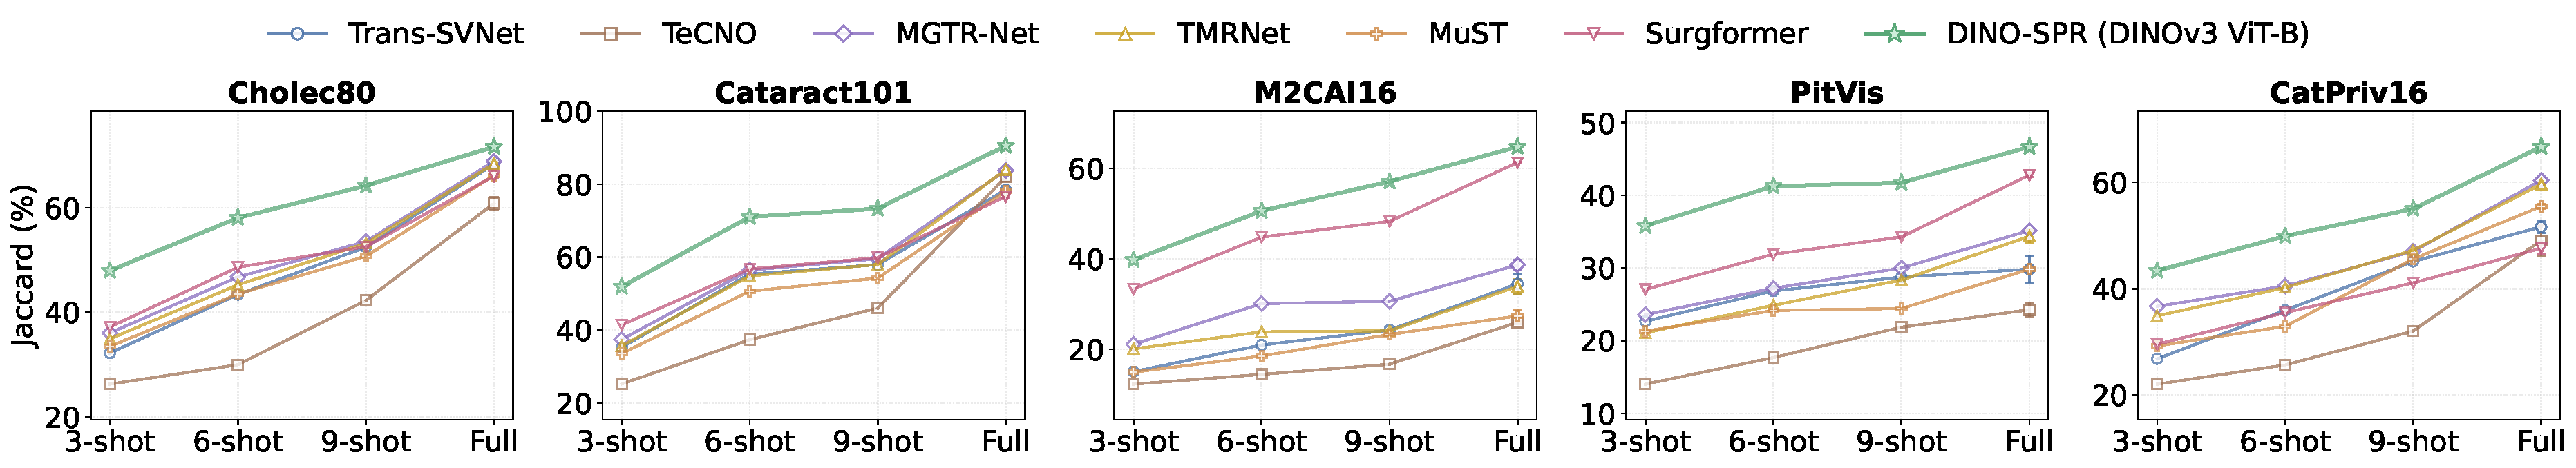
\includegraphics[width=\textwidth]{resources/fig_all_few_shot_trends_full.pdf}
    \caption{Few-shot trends (3-/6-/9-shot) of SPR-Teacher and prior methods on Jaccard, averaged over five datasets.}
    \label{fig:few-shot}
\end{figure*}

\subsection{Evaluation}
\subsubsection{Datasets}
% 5个数据集，覆盖3种手术类型（腹腔镜/眼科/神经外科），公开+私有联合评估。
% 对照 tab_dataset_description 过一遍关键数字即可，不做逐个介绍。
% 要点：(1) 公开数据集(Cholec80/M2CAI16/Cataract101/PitVis)作为行业标准baseline；
%       (2) 私有数据集(CatPriv16)评估跨中心泛化，无数据泄漏风险；
%       (3) 所有视频采样至1fps，few-shot split用3/6/9个标注视频。

To evaluate across diverse surgical scenarios, we curate five SPR
datasets spanning three procedure types: laparoscopic cholecystectomy (Cholec80,
M2CAI16), cataract surgery (Cataract101, CatPriv16), and transsphenoidal pituitary
surgery (PitVis), as summarized in Table~\ref{tab:datasets}. Among them,
CatPriv16 is our private dataset providing a
fully unseen reference for surgical FMs. All videos are sampled at
1\,fps, and few-shot splits use 3, 6, or 9 labeled training videos with unchanged
validation and test sets.

\subsubsection{Metrics}
% 一、SPR 主指标（unrelaxed evaluation）：
%   - 严格逐帧评估（unrelaxed / strict frame-by-frame），不做 temporal smoothing。
%   - 5个 macro-averaged metrics：Accuracy, Precision, Recall, F1, Jaccard。
%   - 均报告 mean±std over 3 seeds。
%   - 首推 Jaccard 作为主指标（最严格、最全面反映帧级分类质量）。
%
% 二、跨数据集一致性：
%   - mean Jaccard：多数据集平均，↑ 越高越好。
%   - Δ = max − min：跨数据集波动，↓ 越低表示泛化越均衡。
%
% 三、效率指标（对照 tab:efficiency，整表 CPU 单核口径）：
%   - Params (M)：部署网络总参数量，↓ 越低越好。
%   - GFLOPs：每帧计算量（backbone only，temporal overhead <0.1G），↓ 越低越好。
%   - FPS：forward-only 吞吐量，fp32、T=8 clip、单核 AMD EPYC 7543，↑ 越高越好。

Following prior work~\cite{jin2021temporal,yang2024surgformer}, we report accuracy,
precision, recall, F1-score, and Jaccard under unrelaxed evaluation, averaged over
three random seeds. We prioritize Jaccard for jointly penalizing frame-level false
positives and negatives, and summarize cross-dataset results by the mean Jaccard
together with the range $\Delta=\max-\min$, where a smaller $\Delta$ indicates more
balanced generalization. For deployment efficiency, we additionally report the
parameter count, per-frame GFLOPs, and the FPS of a single $T{=}8$ clip measured
on a single core of an AMD EPYC 7543 CPU.


\subsection{Comparisons with SOTAs}
\subsubsection{Few-shot Settings}
% 对照 tab_sota_6shot + fig_few_shot_trends：
%
% 1. SOTA 概览：
%   - 现有方法分两类：multi-stage（Trans-SVNet/MGTR-Net/TMRNet/MuST，ResNet50+时序）
%     和 end-to-end（Surgformer，3D ViT+HTA）。
%   - 6-shot 下 prior 方法 Jaccard 最高仅 56.8（Surgformer 在 Cat101），且跨数据集波动大。
%   - Multi-stage 方法依赖分步特征提取（数据量稀缺场景下无法充分微调特征提取器就会导致效果不佳，end-to-end Surgformer 精度尚可但极慢，CPU 单核仅 2.7 FPS）。
%
% 2. DINO-SPR 6-shot 表现（tab_sota_6shot）： ref这个 \label{tab:6shot}
%   - 5 数据集全部指标全面领先，Jaccard 相对最强 prior 高 5.8-14.2 点。
%   - 举具体例子：Cholec80 58.1 vs best SOTA 48.6，Cataract101 71.0 vs 56.8，
%     CatPriv16 49.9 vs 40.5，M2CAI16 50.6 vs 44.8。
%   - 单遍端到端 vs SOTA 两阶段，计算效率对比见 §comp cost。
%
% 3. Few-shot trend（fig_few_shot_trends）： ref这个 \label{fig:few-shot}
%   - 3/6/9-shot 全区间一致领先，DINO-SPR 6-shot 已超 SOTA 9-shot。
%   - 随 shot 数减少，SOTA 急剧下降（e.g. Trans-SVNet Cat101: 9-shot 42→3-shot 26），
%     DINO-SPR 下降平缓（78→55），体现 FM 先验对少样本的鲁棒性。
%   - 举 1-2 个数据集的 trend 例子。

We compare DINO-SPR with eight prior methods spanning two paradigms.
Multi-stage methods, namely Trans-SVNet~\cite{gao2021trans},
TeCNO~\cite{czempiel2020tecno}, MGTR-Net~\cite{huang2025multi},
TMRNet~\cite{jin2021temporal}, MuST~\cite{perez2024must}, LoViT~\cite{liu2025lovit},
and SKiT~\cite{liu2023skit}, fine-tune a backbone before appending a temporal
model. Surgformer~\cite{yang2024surgformer}, the only end-to-end approach, instead
jointly models multiple input frames through spatiotemporal attention in a ViT.
Tables~\ref{tab:6shot_public} and~\ref{tab:6shot_private} report the 6-shot
comparison over the four public datasets and our private CatPriv16, respectively.

Under few-shot supervision, multi-stage methods generally lag behind, since scarce
labels do not allow their feature extractors to be fine-tuned well, whereas the
end-to-end Surgformer performs somewhat better. Leveraging the strong pretraining of
DINOv3 and our few-shot specific spatiotemporal adaptation, DINO-SPR clearly
surpasses all prior methods on every metric and dataset, reaching 58.1, 71.0, and
49.9 Jaccard on Cholec80, Cataract101, and CatPriv16. These scores improve on the
strongest prior method by 9.5, 14.2, and 9.4 on each dataset, and the gains span
5.8 to 14.2 across the five datasets. Figure~\ref{fig:few-shot} further shows that
DINO-SPR leads by a large margin at every label budget. 
The advantage is largest at the extreme 3-shot setting, for instance on M2CAI16,
where DINO-SPR reaches 39.7 Jaccard while the prior method TeCNO falls to
12.3, demonstrating that our method fully exploits the potential of foundation
models.


% VFM backbone-selection ablation (backbone comparison figure)
\begin{figure*}[!hb]
    \centering
    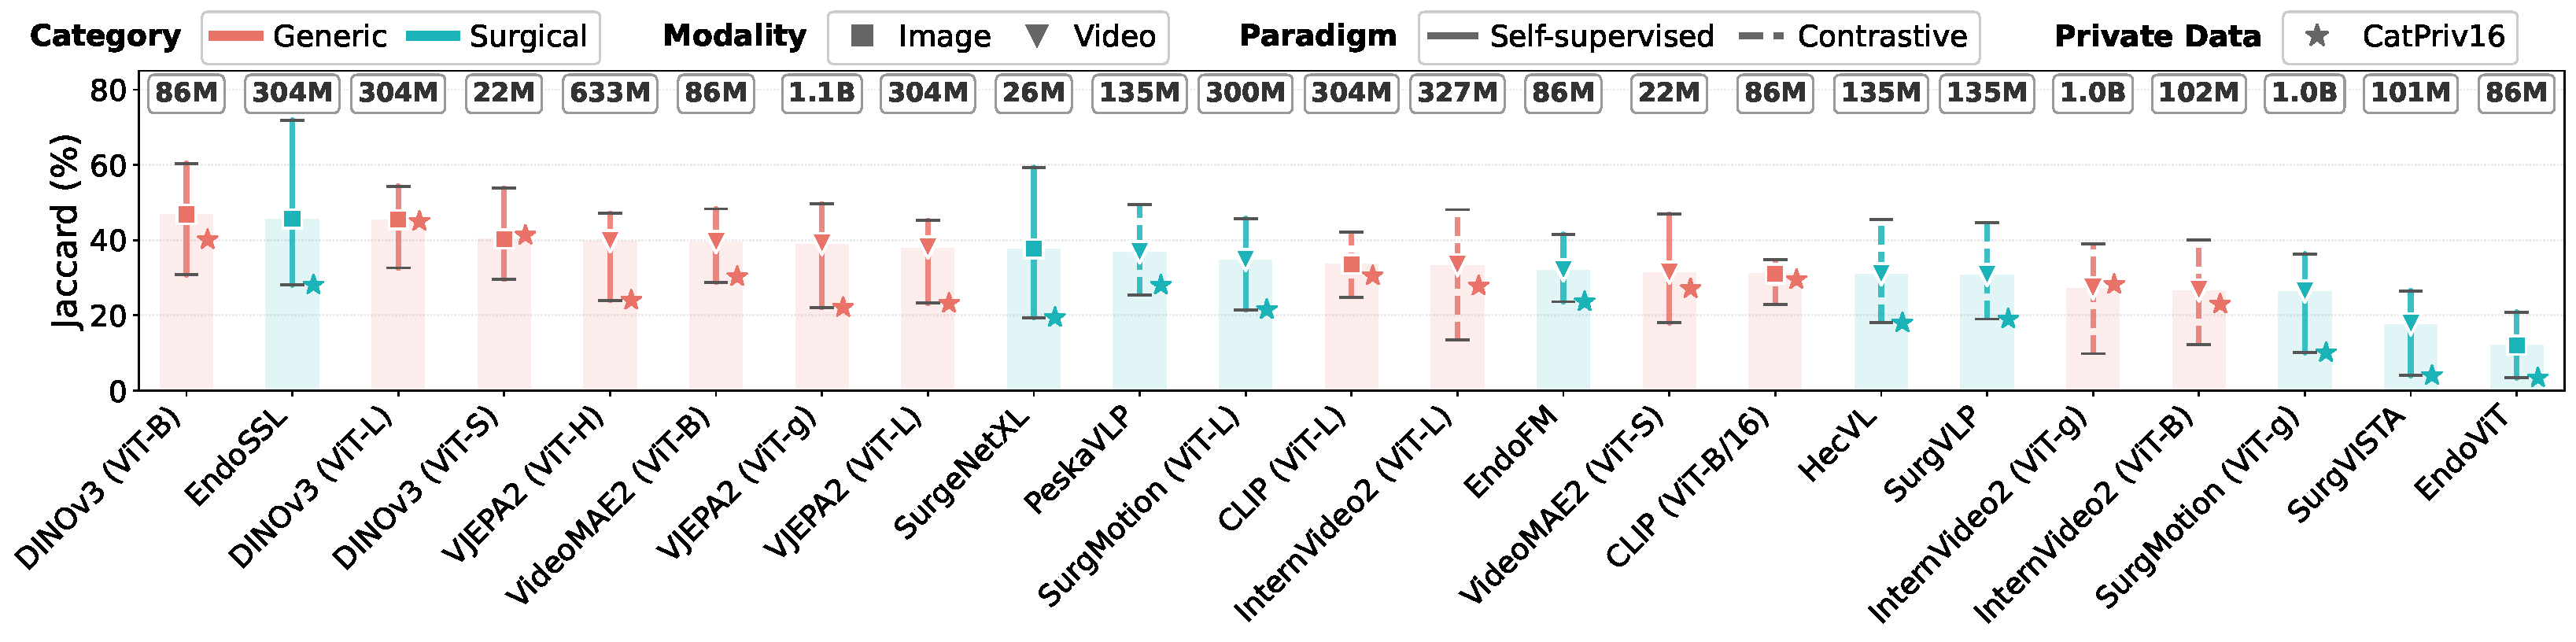
\includegraphics[width=\textwidth]{resources/fig_vfm_backbone.pdf}
    \caption{Ablation of foundation models as the frozen backbone under 6-shot surgical phase recognition with MGTR-Net as the temporal model. For each foundation model, sorted by decreasing mean Jaccard, the vertical bar spans the min--max Jaccard across the five datasets, and the shape marker marks the mean Jaccard. The star marks the private CatPriv16 dataset as an unseen domain, and the labeled value is the parameter size.}
    \label{fig:vfm_backbone}
\end{figure*}



\subsubsection{Computational Cost and Parameter Efficiency}
% 对照 tab_efficiency（整表已改为 CPU 单核口径）：
%
% 1. SOTA 效率问题：
%   - Multi-stage 方法：两遍推理（ResNet50 逐帧提特征 → 时序模型），无法流式处理；
%     ResNet50 前端本身就卡死在 ~8 FPS（Trans-SVNet 8.3 / MGTR-Net 8.2 / MuST 8.4）。
%   - Surgformer：端到端但 121M ViT，CPU 上最慢，仅 2.7 FPS。
%   - SOTA 准确率低（43-49 J）且效率差，难以实际部署。
%
% 2. DINO-SPR：精度最高（58.1 J），但同为 ViT，CPU 上 2.6 FPS、不比 Surgformer 快
%   → 由此引出「精度高 ≠ 可部署」这个动机，再转入蒸馏。
%
% 3. DINO-SPR Lite：异构蒸馏，按目标硬件挑 backbone。
%   - 关键结论：过 25 FPS 线的两个都是 CNN（ConvNeXt-Atto 43.7、StarNet-S4 26.0），
%     而同量级的 ViT 学生 TinyViT-5M 只有 18.6 —— 速度不自动跟着尺寸走。
%   - 待办：图 fig_computational_cost 仍是 GPU/Cataract101 口径，与本节的 CPU 口径不一致。

Clinical deployment often has to work without a dedicated GPU, so we emulate such a
limited environment by measuring all inference on a single CPU core, as reported in
Table~\ref{tab:efficiency} for 6-shot Cholec80.
Prior methods were not designed for real-time inference, and their FPS
only spans 2.7 to 8.4, far below the 25\,FPS native video rate.
Surgformer is the slowest because it jointly attends over all frames of a clip with
a 121M ViT.
DINO-SPR reaches 58.1 Jaccard, yet as a ViT it inherits the same limit
and runs at 2.6\,FPS.
High performance alone thus does not make a model deployable.
Architecture-agnostic distilling DINO-SPR into lightweight students closes that gap and meets the real-time requirement, reaching up to
44\,FPS on a single CPU with performance close to DINO-SPR.

% Efficiency comparison — measured on a single CPU core (AMD EPYC 7543).
% Forward-only, fp32, T=8 clip, batch 1, fps = T / (clip_latency_s),
% median over rounds; raw clip_ms in latex/resources/:
%   cpu_throughput_deployed.json  (Lite rows: deployed DistillStudent, 7x30)
%   cpu_throughput_sota.json      (two-stage rows: ResNet50 + temporal, 5x20)
%   cpu_throughput_final.json     (Surgformer / DINOv3 ViT-B surrogates)
% Params are whole-model counts (backbone + temporal + head) for the Lite rows
% and for Trans-SVNet (25.1M) / MGTR-Net (46.6M).  MuST is the exception: its
% 68.0M is the reported four-stage pipeline (MViT + MTFE + TCM), whereas the
% FPS comes from the ResNet50 surrogate actually timed here (37.2M).
% GFLOPs count the backbone only (temporal overhead <0.1 G).
% Full-node (64-thread) runs excluded: external load on the shared node made
% small-model values swing 2-256 fps.
% The two-stage rows are two-pass pipelines (ResNet50 features precomputed for
% the whole video), so their FPS is a compute rate, not a streaming rate.
\begin{table}[t]
\centering
\caption{Computational cost and performance on 6-shot Cholec80.}
\label{tab:efficiency}
\setlength{\tabcolsep}{3.0pt}
\footnotesize
\begin{tabular}{@{}l@{\hspace{2pt}}r r r r@{}}
\toprule
\textbf{Method} & \textbf{Params}$\downarrow$ & \textbf{GFLOPs}$\downarrow$ & \textbf{FPS}$\uparrow$ & \textbf{Jaccard}$\uparrow$ \\
\midrule
\multicolumn{5}{l}{\textbf{Prior SOTA}} \\
\quad Trans-SVNet        & 25.1M  & 4.1  & 8.3  & 43.4 \\
\quad MGTR-Net           & 46.6M  & 4.1  & 8.2  & 46.7 \\
\quad MuST               & 68.0M  & 10.6 & 8.4  & 43.5 \\
\quad Surgformer         & 121.3M & 22.5 & 2.7  & 48.6 \\
\midrule
\multicolumn{5}{l}{\textbf{DINO-SPR}} \\
\quad DINOv3 ViT-B       & 92.0M  & 17.6 & 2.6  & 58.1 \\
\midrule
\multicolumn{5}{l}{\textbf{DINO-SPR Lite}} \\
\quad TinyViT-5M         & 7.1M & 1.2  & 18.6 & 55.4 \\
\quad StarNet-S4         & 8.9M & 1.1  & 26.0 & 55.2 \\
\quad ConvNeXt-Atto      & 5.4M & 0.6  & 43.7 & 52.2 \\
\bottomrule
\end{tabular}
\end{table}




\subsection{Ablation Study}
\subsubsection{Foundation Model Selection}
% 目的：把 FM benchmark 降级为 backbone 选择的 ablation。两段：config + 图要点。
% 实验设定：冻住各 FM 提特征，MGTR-Net 作时序，6-shot 5 数据集，隔离 FM 特征迁移性。
% 图要点：mean/range/CatPriv16/params；通用 FM 优于手术 FM；DINOv3 是最优起点。

To investigate how FMs generalize to few-shot SPR, we freeze each FM as a
feature extractor and train MGTR-Net~\cite{huang2025multi} as the temporal model on
8-frame windows, under the unified 6-shot protocol across five datasets.
Since surgical FMs may have seen the evaluation datasets during pretraining, we
highlight our private CatPriv16 as a leakage-free reference for fair generalization.

Figure~\ref{fig:vfm_backbone} ranks all FMs by mean Jaccard.
General FMs achieve higher Jaccard with more stable cross-dataset
generalization than surgical FMs.
The instability of surgical FMs likely stems from their pretraining data covering
certain procedure types more thoroughly. On the leakage-free CatPriv16, surgical FMs
nearly all rank at their worst, suggesting their true generalization is weaker than
their inflated scores imply.
By pretraining paradigm, SSL methods outperform contrastive ones, as SSL steers the
model toward spatial details while the contrastive objective is more global and thus
less suited to the spatially discriminative nature of SPR.
Video input does not clearly surpass image input, while incurring a larger
computational burden and parameter count. For instance, VideoMAE2 ViT-g with 1B parameters reaches
47.2, only marginally above the 86M DINOv3 ViT-B at 46.9.
We therefore adopt DINOv3~\cite{simeoni2025dinov3} as the backbone, as it exhibits
strong generalization despite having seen almost no surgical data during pretraining.

% VFM configuration summary (single-column, one row per method)
\begin{table}[t]
\centering
\caption{Configurations of the compared foundation models.}
\label{tab:vfm_config}
\setlength{\tabcolsep}{1.2pt}
\footnotesize
\begin{tabular}{@{}l@{\hspace{12pt}}llll@{}}
\toprule
\multicolumn{1}{l}{\textbf{Method}} & \multicolumn{1}{c}{\textbf{Backbone}} & \multicolumn{1}{c}{\textbf{Paradigm}} & \multicolumn{1}{c}{\textbf{Modality}} & \multicolumn{1}{c}{\textbf{Data}} \\
\midrule
\multicolumn{5}{@{}l}{\textbf{General FMs}} \\
DINOv3 & ViT & DINO & I & 1.7B images \\
CLIP & ViT & CTR & I+T & 400M images \\
VideoMAE2 & ViT & MAE & V & 1.35M videos \\
VJEPA2 & ViT & JEPA & V & 2M videos \\
InternVideo2 & ViT & MAE+CTR & V+T & 1.1M videos \\
\midrule
\multicolumn{5}{@{}l}{\textbf{Surgical FMs}} \\
EndoSSL & ViT & MSN & I & 23.3M images \\
SurgeNetXL & CAFormer & DINO & I & 4.7M images \\
EndoViT & ViT & MAE & I & 744K images \\
SurgMotion & ViT & JEPA & V & 15M videos \\
EndoFM & ViT & MAE & V & 33K videos \\
SurgVISTA & ViT & MAE & V & 3.7K videos \\
PeskaVLP & ResNet+BERT & CTR & V+T & 1.3K videos \\
HecVL & ResNet+BERT & CTR & V+T & 1.3K videos \\
SurgVLP & ResNet+BERT & CTR & V+T & 1.3K videos \\
\bottomrule
\end{tabular}
\vspace{3pt}
\begin{spacing}{0.95}
\footnotesize
I/V/T denotes image/video/text. MAE, DINO, JEPA, and MSN belong to self-supervised learning, while CTR is contrastive learning.
\end{spacing}
\end{table}



\subsubsection{DINOv3 Pretraining and Scale}
% 对照 tab_dinov3_finetune：
%   - 同 ViT-B 架构下对比 Random / IN-1K / DINOv3 三种预训练权重 + Frozen / Finetune 两种模式。
%   - DINOv3 + Finetune 在所有 shot 下均为最优，显著优于 IN-1K + Finetune。
%   - 跨规模对比：ViT-S/B/L，ViT-B 在效果与效率之间最佳平衡，选为主干。
%   - Random 仅保留 Finetune 对照；其表现远落后预训练权重，说明预训练先验不可或缺。
To understand DINOv3's promising few-shot performance, we first probe
the backbone with single frames ($T{=}1$), before adding any temporal module.
Table~\ref{tab:dinov3_finetune} reports this ablation, from which three findings
emerge.
First, pretraining largely decides the outcome, with Jaccard climbing steadily from
random to ImageNet-1K to DINOv3 weights even when the features are frozen.
Fine-tuned DINOv3 ViT-B reaches 48.6 Jaccard on Cholec80 at 6-shot, versus 42.9 for
ImageNet-1K.
Second, scaling yields diminishing returns beyond ViT-B.
Moving from ViT-S to ViT-B brings clear gains, whereas ViT-L improves only marginally
at 3.5$\times$ the parameters (304M versus 86M).
Third, fine-tuning consistently outperforms frozen features.
These findings lead us to adopt DINOv3 ViT-B for its accuracy-efficiency balance and
to fine-tune it in all subsequent experiments.


% DINOv3 Fine-tune vs Frozen Ablation with Pretraining Controls --- Single Column
% T=1 (single frame), Jaccard only.
\begin{table}[t]
\centering
\caption{Backbone pretraining and fine-tuning ablation at T$=$1 (single frame).
We compare random, ImageNet-1K, and DINOv3 weights under frozen and fine-tuned modes across ViT sizes.}
\label{tab:dinov3_finetune}
\footnotesize
\setlength{\tabcolsep}{2.4pt}
\begin{tabular}{@{}l l|rrr|rrr@{}}
\toprule
\multirow{2}{*}{Weights} & \multirow{2}{*}{Mode} & \multicolumn{3}{c}{Cholec80} & \multicolumn{3}{c}{Cataract101} \\
\cmidrule(lr){3-5} \cmidrule(lr){6-8}
& & 3-shot & 6-shot & 9-shot & 3-shot & 6-shot & 9-shot \\
\midrule
\multicolumn{8}{l}{\textbf{ViT-S (22M)}} \\
\quad Random  & Finetune & 21.2 & 24.8 & 28.0 & 10.9 & 16.0 & 16.7 \\
\quad IN-1K    & Frozen   & 30.5 & 33.8 & 35.6 & 22.4 & 29.4 & 31.3 \\
\quad IN-1K    & Finetune & 37.8 & 42.9 & 51.7 & 40.2 & 55.8 & 58.4 \\
\quad DINOv3   & Frozen   & 33.0 & 37.2 & 39.7 & 26.8 & 33.7 & 35.5 \\
\quad DINOv3   & Finetune & \textbf{37.4} & \textbf{44.7} & \textbf{51.9} & \textbf{34.7} & \textbf{55.4} & \textbf{55.1} \\
% \quad DINOv3   & LoRA     & 39.7 & 46.9 & 53.4 & 42.5 & 55.5 & 57.7 \\
\midrule
\multicolumn{8}{l}{\textbf{ViT-B (86M)}} \\
\quad Random  & Finetune & 20.3 & 25.4 & 29.3 & 13.1 & 17.8 & 20.3 \\
\quad IN-1K    & Frozen   & 34.0 & 37.5 & 39.7 & 25.7 & 35.2 & 37.2 \\
\quad IN-1K    & Finetune & 37.0 & 42.9 & 50.1 & 42.2 & 57.2 & 58.7 \\
\quad DINOv3   & Frozen   & 35.6 & 38.8 & 42.3 & 26.1 & 34.6 & 35.3 \\
\quad DINOv3   & Finetune & \textbf{40.9} & \textbf{48.6} & \textbf{54.7} & \textbf{40.9} & \textbf{56.9} & \textbf{62.2} \\
% \quad DINOv3   & LoRA     & 39.1 & 47.8 & 54.7 & 42.9 & 57.1 & 60.2 \\
\midrule
\multicolumn{8}{l}{\textbf{ViT-L (304M)}} \\
\quad Random  & Finetune & 21.0 & 26.2 & 31.3 & 14.5 & 19.9 & 22.0 \\
\quad IN-1K    & Frozen   & 33.2 & 41.3 & 43.0 & 31.9 & 43.3 & 46.2 \\
\quad IN-1K    & Finetune & 37.2 & 44.4 & 49.4 & 45.9 & 56.5 & 56.7 \\
\quad DINOv3   & Frozen   & 36.2 & 42.0 & 45.0 & 26.2 & 35.0 & 36.4 \\
\quad DINOv3   & Finetune & \textbf{42.7} & \textbf{49.7} & \textbf{55.3} & \textbf{47.3} & \textbf{61.8} & \textbf{63.0} \\
% \quad DINOv3   & LoRA     & 44.1 & 48.7 & 57.6 & 46.2 & 60.0 & 60.4 \\
\bottomrule
\end{tabular}
\end{table}

% Spatiotemporal Design Ablation --- Single Column
% Control-variable, 3 progressive regions on DINOv3 ViT-B, 6-shot, Jaccard (J), 1 decimal.
% Gains vs. region baseline in parentheses. R1 baseline: Frozen DINOv3 (CLS).
% R2/R3 baseline: Frozen+LoRA+SSTS (best of R1).
\begin{table}[!ht]
\centering
\caption{Spatiotemporal design ablation on 6-shot training.}
\label{tab:temporal_modeling}
\small
\setlength{\tabcolsep}{3pt}
\begin{tabular}{l c c c}
\toprule
Method & T & Cataract101 & Cholec80 \\
\midrule
\multicolumn{4}{l}{\textbf{R1. Single frame (T=1): spatial design}} \\
\quad Frozen DINOv3 (CLS)              & 1  & 34.6            & 38.8 \\
\quad Fine-tuned DINOv3 (full)       & 1  & 55.0 {\scriptsize (+20.4)} & 46.1 {\scriptsize (+7.3)} \\
\quad Frozen + LoRA (CLS)            & 1  & 55.2 {\scriptsize (+20.6)} & 45.5 {\scriptsize (+6.7)} \\
\quad Frozen + LoRA + mean-patch     & 1  & 53.0 {\scriptsize (+18.4)} & 45.8 {\scriptsize (+7.0)} \\
\quad Frozen + LoRA + SSTS (ours)    & 1  & \textbf{57.7 {\scriptsize (+23.1)}} & \textbf{49.6 {\scriptsize (+10.8)}} \\
\midrule
\multicolumn{4}{l}{\textbf{R2. Simple temporal fusion}} \\
\quad Frozen+LoRA+SSTS (T=1)          & 1  & 57.7            & 49.6 \\
\quad + Mean Pooling   & 4  & 57.8 {\scriptsize (+0.1)}  & 49.8 {\scriptsize (+0.2)} \\
\quad + Mean Pooling   & 8  & 58.2 {\scriptsize (+0.5)}  & 51.2 {\scriptsize (+1.6)} \\
\quad + Max Pooling    & 4  & 61.5 {\scriptsize (+3.8)}  & 49.0 {\scriptsize (-0.6)} \\
\quad + Max Pooling    & 8  & 62.8 {\scriptsize (+5.1)}  & 51.5 {\scriptsize (+1.9)} \\
\quad + Bi-LSTM        & 4  & 60.2 {\scriptsize (+2.5)}  & 52.0 {\scriptsize (+2.4)} \\
\quad + Bi-LSTM        & 8  & \textbf{65.0 {\scriptsize (+7.3)}}  & \textbf{53.5 {\scriptsize (+3.9)}} \\
\midrule
\multicolumn{4}{l}{\textbf{R3. Spatiotemporal fusion (ours)}} \\
\quad Frozen+LoRA+SSTS (T=1)          & 1  & 57.7            & 49.6 \\
\quad + KPTF           & 4  & 64.6 {\scriptsize (+6.9)}  & 53.9 {\scriptsize (+4.3)} \\
\quad + KPTF           & 8  & 71.0 {\scriptsize (+13.3)}  & \textbf{58.1 {\scriptsize (+8.5)}} \\
\quad + KPTF           & 16 & \textbf{76.1 {\scriptsize (+18.4)}}  & 57.3 {\scriptsize (+7.7)} \\
\bottomrule
\end{tabular}
\end{table}



\subsubsection{Different Spatiotemporal Modeling}
% 对照 tab_temporal_modeling：
%   - R1（单帧 T=1）：Frozen DINov3 CLS 仅 38.8/34.6；LoRA 微调涨至 45.5/55.2；
%     LoRA + SSTS 达到 49.6/57.7，验证 SSTS 空间注意力有效性。
%   - R2（简单时序融合）：增加 T 普遍带来增益；Mean/Max Pooling 过于 naive；
%     Bi-LSTM 简单有效，T=8 时涨至 53.5/65.0。
%   - R3（KPTF）：进一步涨至 58.1/71.0（T=8），T=8 为效率与效果平衡点。
Table~\ref{tab:temporal_modeling} ablates spatial and temporal design choices on
Cholec80 and Cataract101 at 6-shot, from single frames to full temporal fusion.
In R1, we freeze the DINOv3 backbone and fine-tune a linear classifier on its CLS
token, which yields only 38.8 and 34.6 Jaccard.
LoRA fine-tuning, which matches full fine-tuning at a fraction of the cost, lifts
Jaccard to 45.5 and 55.2, and our SSTS module further raises it to 49.6 and 57.7,
confirming the value of salient spatial token selection.
In R2, temporal fusion over this R1-best setup adds clear gains as the clip lengthens,
and a lightweight Bi-LSTM is the strongest simple aggregator, reaching 53.5 and 65.0
at T$=$8.
In R3, our KPTF module, which guides temporal fusion by keyframe priors, surpasses
Bi-LSTM at every clip length, reaching 58.1 and 71.0 at T$=$8.
Since longer clips do not necessarily bring further gains, we adopt T$=$8 as the
default.

% Distillation model comparison across three lightweight families, curated students.
% 6-shot, T=8, Jaccard (%). Each data cell: "w/o KD -> w/ KD" (student-only -> CAP + STGD).
% Arrow notation explained in caption; Family labels in region headers.
% Within each family, same-series models grouped together, sorted by parameter count.
% Params are DEPLOYED counts: backbone + student spatial attention + dim adapter +
%   temporal fusion + head (distill3mod stage B), i.e. what actually runs at
%   inference -- not the bare timm backbone.  Measured 2026-09-10; the teacher
%   row keeps its whole-model count.  Note: the MobileOne rows show the
%   training-time (un-reparameterized) form, which is much larger than the
%   fused inference form.
% Commented-out series (distilled accuracy trails same-family alternatives):
%   Pure CNN: MobileNetV3-Large, MobileOne-S1/S2; ViT-based: DeiT-Tiny/Small, RepViT-M1.1.
% 2026-09-05: student-only baselines lowered so a tiny student trained on 6-shot task
%   loss stays below the strongest prior (Surgformer) in each dataset, by -10 Jaccard on
%   Cataract101 and -3 on Cholec80. Distilled (w/ KD) values unchanged.
\begin{table}[b]
\centering
\caption{Distillation of SPR-Teacher into lightweight students on 6-shot settings.
Each cell: student-only $\rightarrow$ distilled.}
\label{tab:distill_models}
\small
\setlength{\tabcolsep}{4pt}
\begin{tabular}{l c c c}
\toprule
Model & Params$\downarrow$ & Cataract101$\uparrow$ & Cholec80$\uparrow$ \\
\midrule
\multicolumn{4}{l}{\textbf{Teacher}} \\
\quad SPR-Teacher (ViT-B)            & 92M  & 71.0            & 58.1 \\
\midrule
\multicolumn{4}{l}{\textbf{Pure CNN}} \\
\quad ConvNeXt-Atto               & 5.4M & 50.2 $\rightarrow$ 71.6 & 39.8 $\rightarrow$ 52.2 \\
\quad ConvNeXt-Tiny               & 33.3M & 53.6 $\rightarrow$ \textbf{72.2}          & 43.3 $\rightarrow$ \textbf{57.8} \\
\quad StarNet-S2                  & 5.1M & 51.3 $\rightarrow$ 69.7          & 36.6 $\rightarrow$ 52.3 \\
\quad StarNet-S4                  & 8.9M & 52.4 $\rightarrow$ 71.7          & 44.2 $\rightarrow$ 55.2 \\
\quad MobileNetV3-Small           & 3.6M & 50.2 $\rightarrow$ 66.8          & 43.1 $\rightarrow$ 53.0 \\
%\quad MobileNetV3-Large           & 7.1M & 37.2 $\rightarrow$ 61.0          & 34.2 $\rightarrow$ 52.3 \\
%\quad MobileOne-S1                & 9.3M & 46.7 $\rightarrow$ 64.9          & 33.6 $\rightarrow$ 52.4 \\
%\quad MobileOne-S2                & 17.4M & 48.1 $\rightarrow$ 69.1          & 34.3 $\rightarrow$ 52.9 \\
\midrule
\multicolumn{4}{l}{\textbf{ViT-based}} \\
\quad TinyViT-5M                  & 7.1M & 45.8 $\rightarrow$ 70.9          & 41.9 $\rightarrow$ 55.4 \\
\quad TinyViT-11M                 & 12.8M & 47.5 $\rightarrow$ \textbf{72.3}          & 45.0 $\rightarrow$ \textbf{57.5} \\
\quad RepViT-M0.9                 & 6.9M & 45.8 $\rightarrow$ 65.2          & 36.1 $\rightarrow$ 52.0 \\
%\quad RepViT-M1.1                 & 10.2M & 40.2 $\rightarrow$ 66.1          & 37.4 $\rightarrow$ 49.8 \\
%\quad DeiT-Tiny                   & 7.3M & 36.9 $\rightarrow$ 60.2          & 41.5 $\rightarrow$ 51.2 \\
%\quad DeiT-Small                  & 23.8M & 41.8 $\rightarrow$ 63.0          & 42.9 $\rightarrow$ 53.5 \\
\midrule
\multicolumn{4}{l}{\textbf{Hybrid}} \\
\quad MobileViTv2-100             & 6.8M & 47.0 $\rightarrow$ 66.2          & 43.3 $\rightarrow$ 55.4 \\
\quad MobileViTv2-150             & 13.1M & 43.0 $\rightarrow$ \textbf{71.0}          & 35.7 $\rightarrow$ \textbf{55.5} \\
\quad EdgeNeXt-XXS                & 2.9M & 45.6 $\rightarrow$ 67.9          & 37.6 $\rightarrow$ 53.3 \\
\quad EdgeNeXt-XS                 & 4.0M & 48.5 $\rightarrow$ 68.8          & 40.7 $\rightarrow$ 54.7 \\
\bottomrule
\end{tabular}
\end{table}


\subsubsection{Different Lightweight Models for DINO-SPR Lite}
% 对照 tab_distill_models：
%   - CNN / ViT / Hybrid 三类架构通过统一 CAP+STGD 蒸馏，student-only → distilled 均有显著增益。
%   - ConvNeXt-Atto（5.4M 部署口径）蒸馏后 Cat 达 71.6 J，超过 teacher。
%   - 异构蒸馏使部署端可自由选择最适合硬件的 backbone 族。
Table~\ref{tab:distill_models} compares each student trained from scratch and after
architecture-agnostic distillation on Cataract101 and Cholec80.
Distillation improves every mainstream lightweight backbone across the three
architecture categories, by over 20 Jaccard on average on Cataract101, confirming
that it transfers DINO-SPR knowledge to heterogeneous students.
In particular, the strongest student of each family reaches 72.2, 72.3, and 71.0 for
ConvNeXt-Tiny, TinyViT-11M, and MobileViTv2-150, respectively, matching or exceeding
the 92M teacher's 71.0 on Cataract101.
Distillation thus allows picking the backbone best suited to the deployment
setting with little performance loss.

% Distillation ablation, non-cumulative: each component trained alone and jointly.
% Aligned to the overall objective L = L_CE + L_cap + L_stgd (STGD bundles the
% representation, prior, and logit terms). One CNN student (ConvNeXt-Atto,
% heterogeneous, the design target of CAP); two dataset columns. The student-only
% baseline row is kept for reference. Same frozen SPR-Teacher teacher (dsx_bilstm).
% 6-shot, T=8, Jaccard (%). Gains vs. student-only in parentheses.
% src: research_logs/CAP_architecture_agnostic_distillation.md
% 2026-09-05: CE baseline matches the scaled ConvNeXt-Atto no-KD of tab_distill_models
%   (Cataract101 50.2 / Cholec80 39.8); last row = complete scheme = the distilled
%   ConvNeXt-Atto in tab_distill_models. The CAP-only and STGD-only values are
%   placeholders (not re-run); the last row holds the real values.
\begin{table}[t]
\centering
\caption{Distillation design ablation on 6-shot setting.}
\label{tab:distill_strategy}
\small
\setlength{\tabcolsep}{5pt}
\begin{tabular}{l c c}
\toprule
ConvNeXt-Atto (CNN) & Cataract101 & Cholec80 \\
\midrule
Student only (w/o distillation)                & 50.2                   & 39.8                   \\
+ $L_\mathrm{cap}$ (CAP only)                 & 62.4 {\scriptsize (+12.2)} & 47.0 {\scriptsize (+7.2)} \\
+ $L_\mathrm{stgd}$ (STGD only)               & 59.0 {\scriptsize (+8.8)} & 44.8 {\scriptsize (+5.0)} \\
+ $L_\mathrm{cap}$ + $L_\mathrm{stgd}$ (Full method) & 71.6 {\scriptsize (+21.4)} & 52.2 {\scriptsize (+12.4)} \\
\bottomrule
\end{tabular}
\end{table}



\subsubsection{Different Distillation Strategies}
% 对照 tab_distill_strategy（CNN 学生 ConvNeXt-Atto）：
%   - 非累积消融，行标签用 method 顶层 loss term：student-only($L_{CE}$) 参照行 +
%     单独 $L_{cap}$(CAP)、单独 $L_{stgd}$(STGD)、$L_{cap}$+$L_{stgd}$(完整)。
%   - baseline 与 tab_distill_models 的 Atto no-KD 对齐（50.2/39.8，已按 SOTA 下调）；末行=71.6/52.2。
%   - CAP/STGD 单独值为占位（未重跑），末行与 tab_distill_models 的 distilled 一致。
We ablate the distillation components on the heterogeneous CNN ConvNeXt-Atto in
Table~\ref{tab:distill_strategy}. Training with the task loss $L_\mathrm{CE}$ alone stays
weak at 50.2 on Cataract101, because the scarce labels offer little supervision
to the small model. Adding $L_\mathrm{cap}$ alone improves it to 62.4, a larger
gain than $L_\mathrm{stgd}$ alone at 59.0, which shows that bridging the
representation gap matters most. Combining the two lifts the result substantially to
71.6, and Cholec80 follows the same trend, rising to 52.2 from the 39.8 baseline.


\begin{figure}[b]
    \centering
    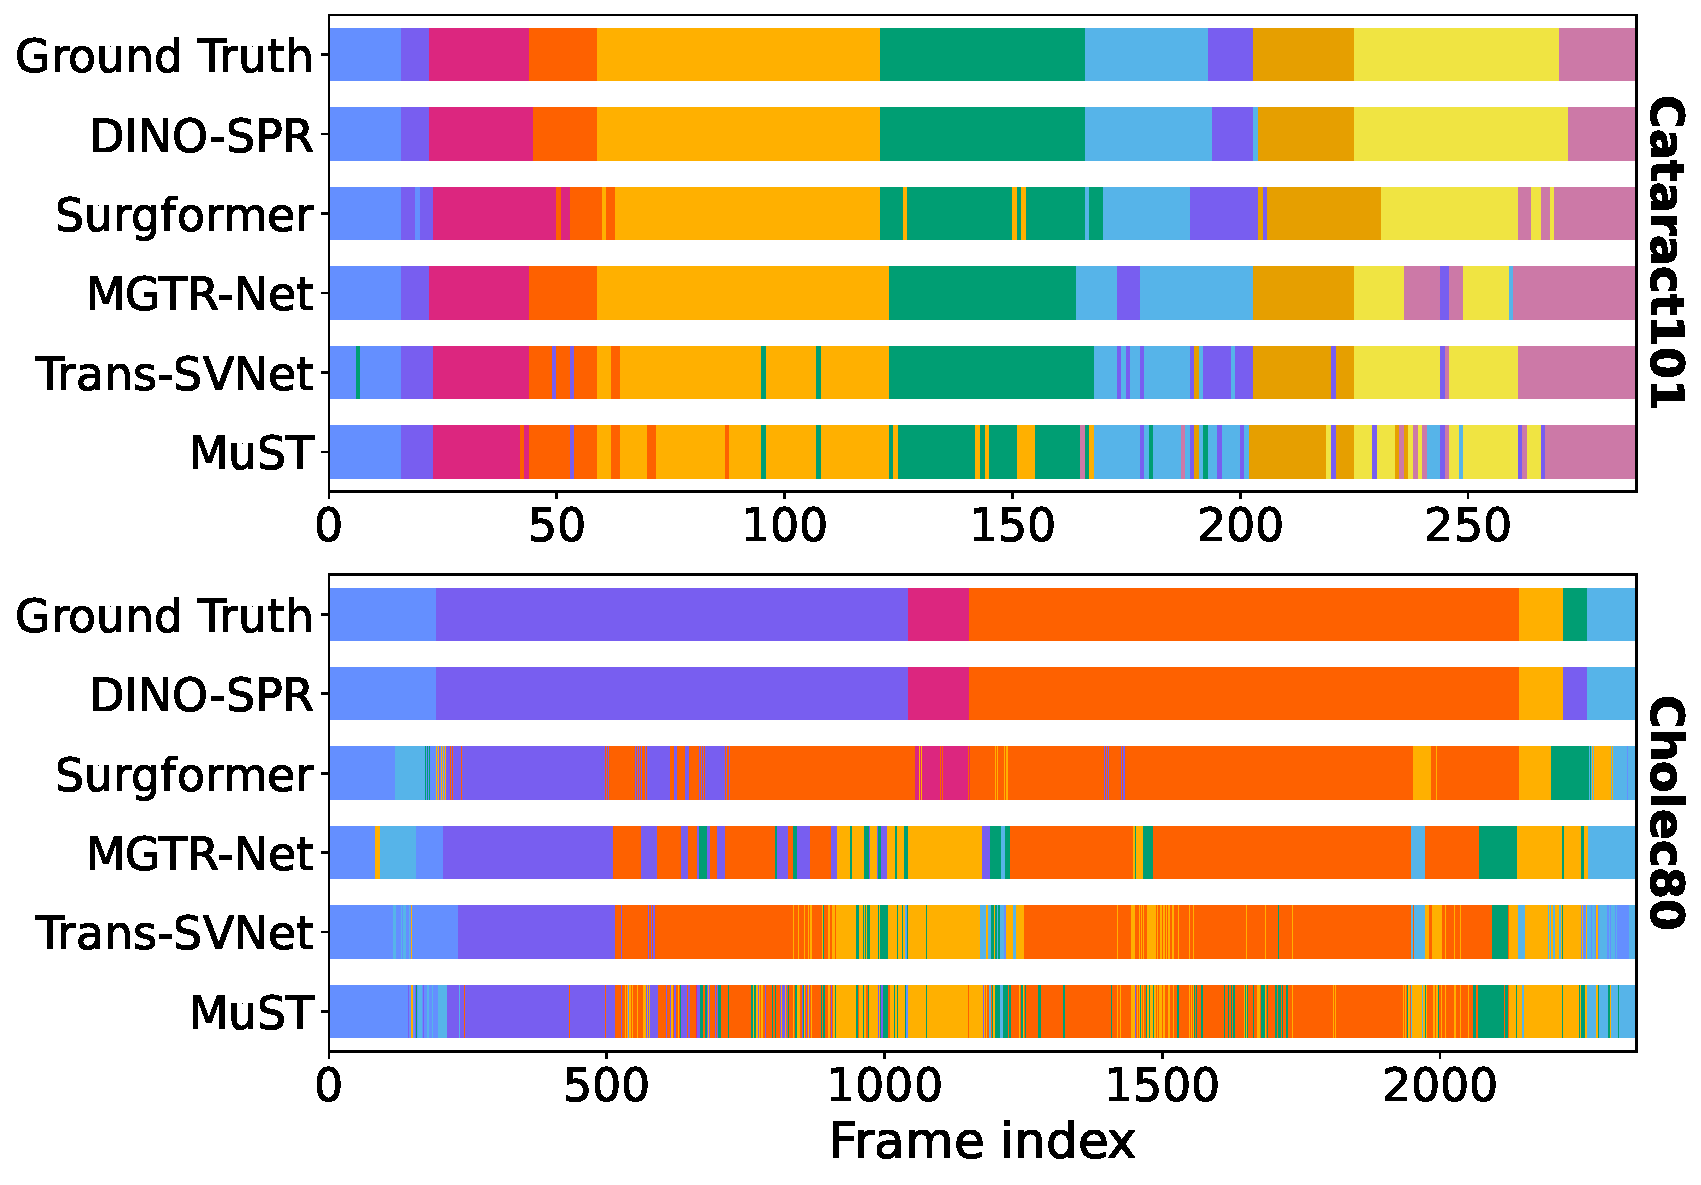
\includegraphics[width=\columnwidth]{resources/fig_phase_comparison_final_nolegend.pdf}
    \caption{Per-frame phase predictions of SPR-Teacher versus prior methods under the 6-shot setting on Cholec80 and Cataract101.}
    \label{fig:phase}
\end{figure}
\begin{figure*}[!ht]
    \centering
    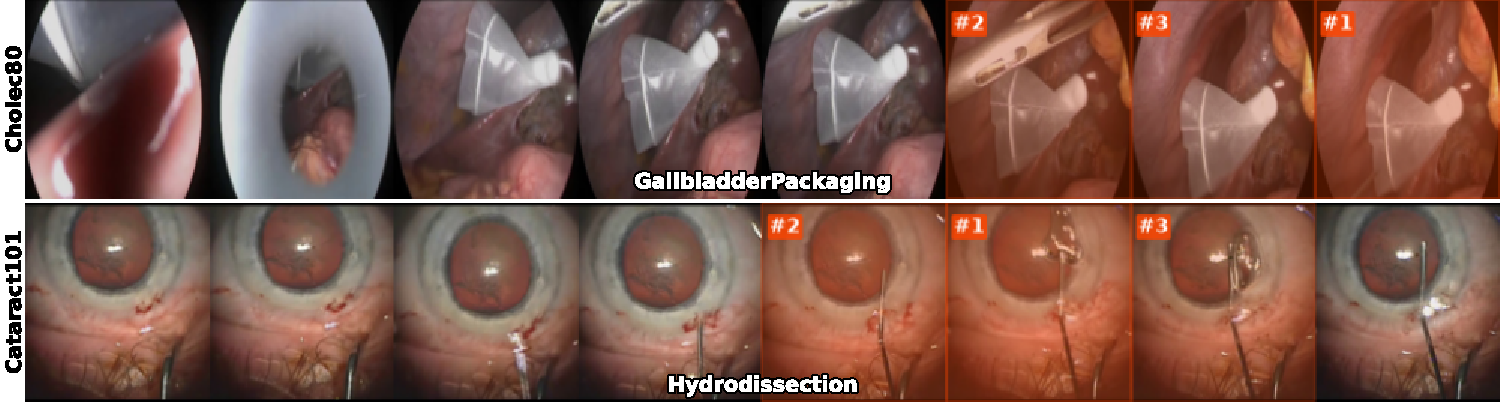
\includegraphics[width=\textwidth]{resources/temporal_final.pdf}
    \caption{Keyframe selection of the KPTF module. Within an 8-frame window, the top-3 frames with the largest temporal weights are highlighted (\#1--\#3); KPTF prioritizes frames with salient instrument-tissue interactions, which carry the strongest discriminative evidence.}
    \label{fig:keyframe}
\end{figure*}
\begin{figure}[!h]
    \centering
    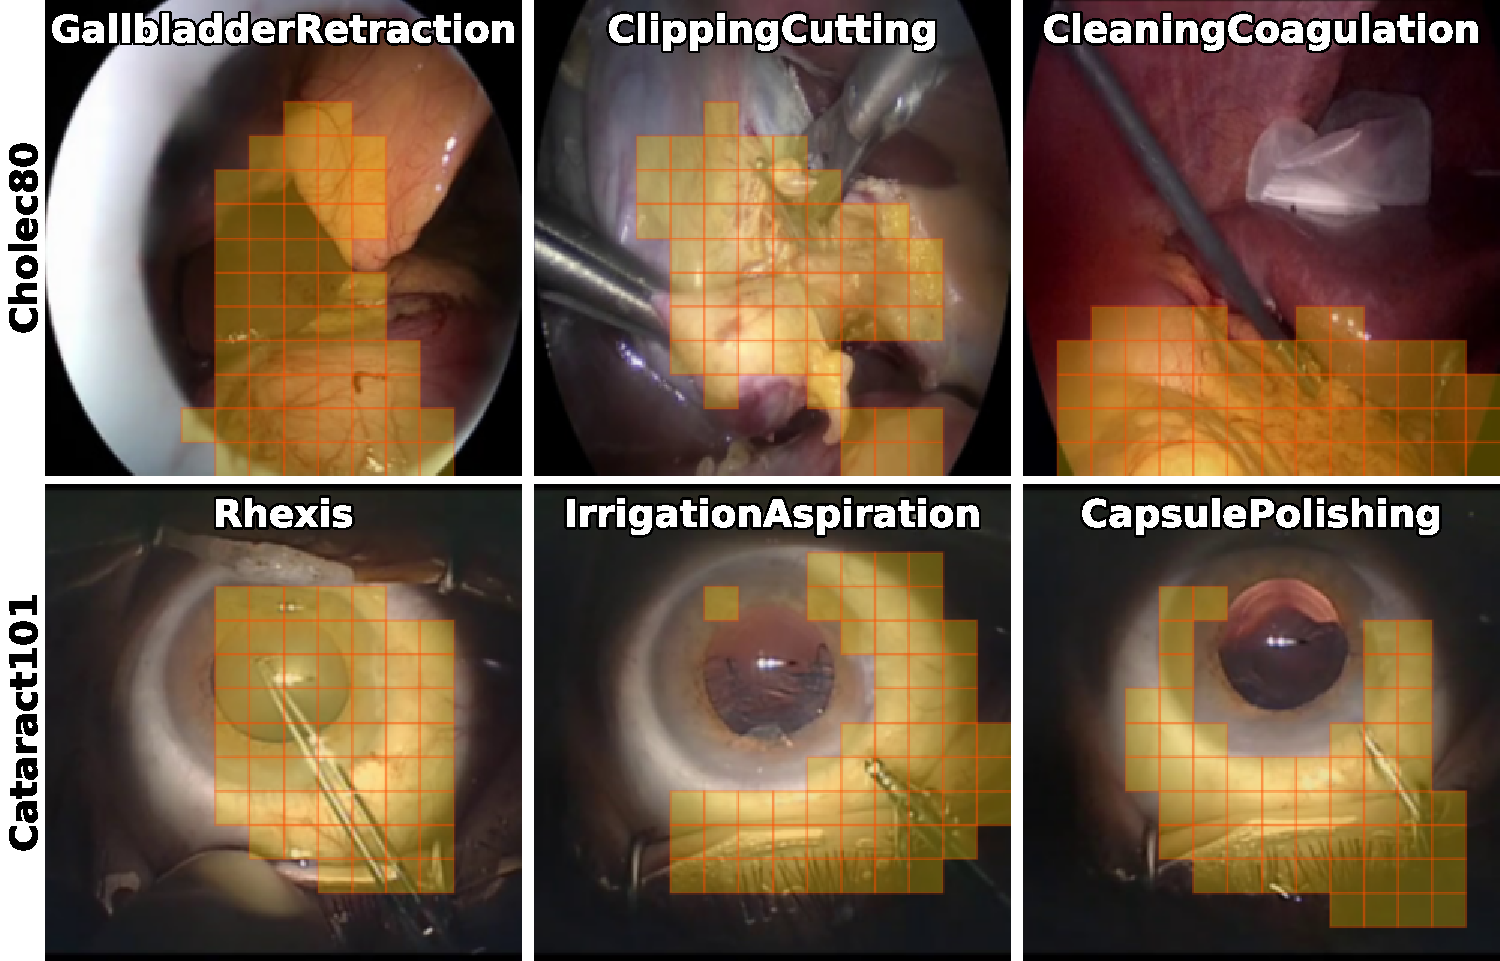
\includegraphics[width=\columnwidth]{resources/spatial_final.pdf}
    \caption{Spatial token selection of the SSTS module. Selected tokens (yellow) focus on instrument-tissue interactions while suppressing background, revealing the saliency prior guiding phase discrimination.}
    \label{fig:spatial}
\end{figure}


\subsection{Qualitative Analysis}
\subsubsection{Frame-level Phase Recognition}
% ref \label{fig:phase}：SPR 结果更准确，尤其 phase 边界切换、整体连续性、正确 phase 匹配。
Figure~\ref{fig:phase} compares per-frame predictions of DINO-SPR with prior
methods on test videos from Cholec80 and Cataract101.
DINO-SPR produces more continuous and accurate phase recognition, with cleaner boundaries
and far fewer fragmented predictions.
The improvement is most pronounced at phase transitions, where the spatiotemporal
module captures discriminative cues across frames to keep the prediction coherent,
while prior methods oscillate rapidly between adjacent phases.
Overall, the predicted sequences align closely with the ground-truth annotations,
showing that our end-to-end spatiotemporal design keeps accurate recognition even
under the limited supervision.
%
\subsubsection{Spatiotemporal Module Visualization}
% ref \label{fig:keyframe}：关键帧 KPTF weights top-3 highlight，展示 keyframe selection 有效性。
% ref \label{fig:spatial}：SSTS spatial token selection highlight，展示关注器械/组织区域而非背景。
Figure~\ref{fig:keyframe} visualizes the top-3 frames that KPTF selects within the input window.
The selected frames consistently capture informative moments such as
instrument-tissue interaction, while background-dominated views (e.g.,
out-of-focus or instrument-withdrawn scenes) receive low scores.
This shows that KPTF picks discriminative keyframes without explicit
supervision.
Figure~\ref{fig:spatial} visualizes the spatial token selection of SSTS, where
high-scoring patches concentrate on surgical instruments and tissue surfaces rather
than on irrelevant background.
These demonstrate that DINO-SPR focuses on the spatial and temporal
cues that carry the strongest discriminative evidence.






\section{Conclusion and Limitations}
\label{sec:conclusion}

%%% Conclusion 设计要点（正文已写，注释为背景） %%
% 风格：精炼，正文把 conclusion 与 limitations 合并成一段；回扣 intro 的三大卖点，不引入新内容。

%%% 1. 回扣任务与方法（走故事线，避免流水账式总结） %%%
% 动机：FM 范式自身两大临床缺陷——数据饥渴 + 实时性差 → 本文研究 = 修复二者
% 统一视角：手术视频双重冗余（空间背景 + 时间稳态帧）是数据缺陷背后的关键障碍
% 方法：对抗冗余两阶段——
%   修数据缺陷 SPR-Teacher：SSTS 压空间冗余 + KPTF 压时间冗余，冻结 generic FM + 少量标注；
%   修实时缺陷 SPR-Lite：CAP 跨架构 + STGD 时空先验稠密监督。
%   （不复述 generic vs surgical FM 对比——那已降级为引言一句 motivation）
%%% 2. 结果总结（方法 / 部署） %%%
% 方法：SPR-Teacher 在 4 公开 + 1 私有数据集 few-shot 大幅超越 prior SOTA。
% 部署：Lite 保留精度，参数大幅压缩、实时性显著提升。
%%% 3. 临床意义 + 未来工作 %%%
% 为低标注、实时可部署的智能手术室提供可行路径；
% 未来：更多术式与多模态、真实临床硬件验证、更强蒸馏目标。

%%% Limitation 设计要点（已并入同一段，正文已写，注释为背景） %%
% 总基调：坦诚、客观，笼统总结，不点名具体模型/数据集，不引用表格，落到"未来可做"上。

%%% 1. 只考虑公开权重的 FM，覆盖不全 %%%
% 后果：所用 FM 的全面性受限。
% 未来：期待社区开放更多权重。

%%% 2. surgical FM 预训练存在手术数据泄露，FM 对比未必公平 %%%
% 事实：surgical FM 不可避免地会在公开手术视频上预训练，部分可能与评测数据重叠、使其分数虚高，
%   故 generic vs surgical 的 FM 对比不完全公平。
% 未来：期待更严格的"未见术式"评估协议。

%%% 3. 实时性未在真实临床硬件上验证 %%%
% 未来：针对临床硬件做量化与工程优化。

Surgical phase recognition is a fundamental task for intelligent operating
rooms. In the foundation model era, its clinical deployment is hindered by
two deficiencies of the FM paradigm itself: a reliance on massive training
data and an inability to infer in real time on clinical hardware. We argue
that the dual redundancy of surgical videos---dominant background regions and
repetitive steady-state frames---is the key obstacle behind the data
deficiency, and propose to combat it in both the model and its
distillation. SPR-Teacher compresses spatial redundancy through salient spatial
token selection and temporal redundancy through keyframe-prior temporal
fusion, adapting a frozen generic foundation model with only a handful of
labeled videos. SPR-Lite then lifts the real-time deficiency by
compressing the model itself, where a
cross-attention projection bridges arbitrary student architectures and a
spatiotemporally-guided distillation transfers the teacher's where- and
when-to-look priors as dense supervision. Across four public and one private
dataset, SPR-Teacher surpasses prior methods under few-shot settings by large
margins, while SPR-Lite retains this performance with under 9M
parameters at over 25\,FPS on a single CPU core, offering a practical route
toward low-annotation, real-time deployment.
Nevertheless, several limitations remain. First, we only consider foundation
models with publicly released
weights, so the coverage may not be exhaustive. Second, surgical FMs
inevitably pre-train on public surgical videos, part of which may overlap with
our evaluation data and inflate their scores, making the FM comparison not
perfectly fair. Third, real-time efficiency is measured on a server CPU core
rather than on clinical hardware, where quantization and further engineering
optimization remain to be explored. We leave these for future work.




\appendices

\section{Configurations of the Compared Foundation Models}
\label{app:vfm_config}
% VFM configuration summary (single-column, one row per method)
\begin{table}[t]
\centering
\caption{Configurations of the compared foundation models.}
\label{tab:vfm_config}
\setlength{\tabcolsep}{1.2pt}
\footnotesize
\begin{tabular}{@{}l@{\hspace{12pt}}llll@{}}
\toprule
\multicolumn{1}{l}{\textbf{Method}} & \multicolumn{1}{c}{\textbf{Backbone}} & \multicolumn{1}{c}{\textbf{Paradigm}} & \multicolumn{1}{c}{\textbf{Modality}} & \multicolumn{1}{c}{\textbf{Data}} \\
\midrule
\multicolumn{5}{@{}l}{\textbf{General FMs}} \\
DINOv3 & ViT & DINO & I & 1.7B images \\
CLIP & ViT & CTR & I+T & 400M images \\
VideoMAE2 & ViT & MAE & V & 1.35M videos \\
VJEPA2 & ViT & JEPA & V & 2M videos \\
InternVideo2 & ViT & MAE+CTR & V+T & 1.1M videos \\
\midrule
\multicolumn{5}{@{}l}{\textbf{Surgical FMs}} \\
EndoSSL & ViT & MSN & I & 23.3M images \\
SurgeNetXL & CAFormer & DINO & I & 4.7M images \\
EndoViT & ViT & MAE & I & 744K images \\
SurgMotion & ViT & JEPA & V & 15M videos \\
EndoFM & ViT & MAE & V & 33K videos \\
SurgVISTA & ViT & MAE & V & 3.7K videos \\
PeskaVLP & ResNet+BERT & CTR & V+T & 1.3K videos \\
HecVL & ResNet+BERT & CTR & V+T & 1.3K videos \\
SurgVLP & ResNet+BERT & CTR & V+T & 1.3K videos \\
\bottomrule
\end{tabular}
\vspace{3pt}
\begin{spacing}{0.95}
\footnotesize
I/V/T denotes image/video/text. MAE, DINO, JEPA, and MSN belong to self-supervised learning, while CTR is contrastive learning.
\end{spacing}
\end{table}


\bibliographystyle{IEEEtran}
\bibliography{mybibliography}

\end{document}
